% Options for packages loaded elsewhere
% Options for packages loaded elsewhere
\PassOptionsToPackage{unicode}{hyperref}
\PassOptionsToPackage{hyphens}{url}
\PassOptionsToPackage{dvipsnames,svgnames,x11names}{xcolor}
%
\documentclass[
  11pt,
  a4paper,
]{article}
\usepackage{xcolor}
\usepackage[margin=2.5cm]{geometry}
\usepackage{amsmath,amssymb}
\setcounter{secnumdepth}{5}
\usepackage{iftex}
\ifPDFTeX
  \usepackage[T1]{fontenc}
  \usepackage[utf8]{inputenc}
  \usepackage{textcomp} % provide euro and other symbols
\else % if luatex or xetex
  \usepackage{unicode-math} % this also loads fontspec
  \defaultfontfeatures{Scale=MatchLowercase}
  \defaultfontfeatures[\rmfamily]{Ligatures=TeX,Scale=1}
\fi
\usepackage{lmodern}
\ifPDFTeX\else
  % xetex/luatex font selection
\fi
% Use upquote if available, for straight quotes in verbatim environments
\IfFileExists{upquote.sty}{\usepackage{upquote}}{}
\IfFileExists{microtype.sty}{% use microtype if available
  \usepackage[]{microtype}
  \UseMicrotypeSet[protrusion]{basicmath} % disable protrusion for tt fonts
}{}
\makeatletter
\@ifundefined{KOMAClassName}{% if non-KOMA class
  \IfFileExists{parskip.sty}{%
    \usepackage{parskip}
  }{% else
    \setlength{\parindent}{0pt}
    \setlength{\parskip}{6pt plus 2pt minus 1pt}}
}{% if KOMA class
  \KOMAoptions{parskip=half}}
\makeatother
% Make \paragraph and \subparagraph free-standing
\makeatletter
\ifx\paragraph\undefined\else
  \let\oldparagraph\paragraph
  \renewcommand{\paragraph}{
    \@ifstar
      \xxxParagraphStar
      \xxxParagraphNoStar
  }
  \newcommand{\xxxParagraphStar}[1]{\oldparagraph*{#1}\mbox{}}
  \newcommand{\xxxParagraphNoStar}[1]{\oldparagraph{#1}\mbox{}}
\fi
\ifx\subparagraph\undefined\else
  \let\oldsubparagraph\subparagraph
  \renewcommand{\subparagraph}{
    \@ifstar
      \xxxSubParagraphStar
      \xxxSubParagraphNoStar
  }
  \newcommand{\xxxSubParagraphStar}[1]{\oldsubparagraph*{#1}\mbox{}}
  \newcommand{\xxxSubParagraphNoStar}[1]{\oldsubparagraph{#1}\mbox{}}
\fi
\makeatother


\usepackage{longtable,booktabs,array}
\newcounter{none} % for unnumbered tables
\usepackage{calc} % for calculating minipage widths
% Correct order of tables after \paragraph or \subparagraph
\usepackage{etoolbox}
\makeatletter
\patchcmd\longtable{\par}{\if@noskipsec\mbox{}\fi\par}{}{}
\makeatother
% Allow footnotes in longtable head/foot
\IfFileExists{footnotehyper.sty}{\usepackage{footnotehyper}}{\usepackage{footnote}}
\makesavenoteenv{longtable}
\usepackage{graphicx}
\makeatletter
\newsavebox\pandoc@box
\newcommand*\pandocbounded[1]{% scales image to fit in text height/width
  \sbox\pandoc@box{#1}%
  \Gscale@div\@tempa{\textheight}{\dimexpr\ht\pandoc@box+\dp\pandoc@box\relax}%
  \Gscale@div\@tempb{\linewidth}{\wd\pandoc@box}%
  \ifdim\@tempb\p@<\@tempa\p@\let\@tempa\@tempb\fi% select the smaller of both
  \ifdim\@tempa\p@<\p@\scalebox{\@tempa}{\usebox\pandoc@box}%
  \else\usebox{\pandoc@box}%
  \fi%
}
% Set default figure placement to htbp
\def\fps@figure{htbp}
\makeatother


% definitions for citeproc citations
\NewDocumentCommand\citeproctext{}{}
\NewDocumentCommand\citeproc{mm}{%
  \begingroup\def\citeproctext{#2}\cite{#1}\endgroup}
\makeatletter
 % allow citations to break across lines
 \let\@cite@ofmt\@firstofone
 % avoid brackets around text for \cite:
 \def\@biblabel#1{}
 \def\@cite#1#2{{#1\if@tempswa , #2\fi}}
\makeatother
\newlength{\cslhangindent}
\setlength{\cslhangindent}{1.5em}
\newlength{\csllabelwidth}
\setlength{\csllabelwidth}{3em}
\newenvironment{CSLReferences}[2] % #1 hanging-indent, #2 entry-spacing
 {\begin{list}{}{%
  \setlength{\itemindent}{0pt}
  \setlength{\leftmargin}{0pt}
  \setlength{\parsep}{0pt}
  % turn on hanging indent if param 1 is 1
  \ifodd #1
   \setlength{\leftmargin}{\cslhangindent}
   \setlength{\itemindent}{-1\cslhangindent}
  \fi
  % set entry spacing
  \setlength{\itemsep}{#2\baselineskip}}}
 {\end{list}}
\usepackage{calc}
\newcommand{\CSLBlock}[1]{\hfill\break\parbox[t]{\linewidth}{\strut\ignorespaces#1\strut}}
\newcommand{\CSLLeftMargin}[1]{\parbox[t]{\csllabelwidth}{\strut#1\strut}}
\newcommand{\CSLRightInline}[1]{\parbox[t]{\linewidth - \csllabelwidth}{\strut#1\strut}}
\newcommand{\CSLIndent}[1]{\hspace{\cslhangindent}#1}



\setlength{\emergencystretch}{3em} % prevent overfull lines

\providecommand{\tightlist}{%
  \setlength{\itemsep}{0pt}\setlength{\parskip}{0pt}}



 


\makeatletter
\@ifpackageloaded{caption}{}{\usepackage{caption}}
\AtBeginDocument{%
\ifdefined\contentsname
  \renewcommand*\contentsname{Table of contents}
\else
  \newcommand\contentsname{Table of contents}
\fi
\ifdefined\listfigurename
  \renewcommand*\listfigurename{List of Figures}
\else
  \newcommand\listfigurename{List of Figures}
\fi
\ifdefined\listtablename
  \renewcommand*\listtablename{List of Tables}
\else
  \newcommand\listtablename{List of Tables}
\fi
\ifdefined\figurename
  \renewcommand*\figurename{Figure}
\else
  \newcommand\figurename{Figure}
\fi
\ifdefined\tablename
  \renewcommand*\tablename{Table}
\else
  \newcommand\tablename{Table}
\fi
}
\@ifpackageloaded{float}{}{\usepackage{float}}
\floatstyle{ruled}
\@ifundefined{c@chapter}{\newfloat{codelisting}{h}{lop}}{\newfloat{codelisting}{h}{lop}[chapter]}
\floatname{codelisting}{Listing}
\newcommand*\listoflistings{\listof{codelisting}{List of Listings}}
\makeatother
\makeatletter
\makeatother
\makeatletter
\@ifpackageloaded{caption}{}{\usepackage{caption}}
\@ifpackageloaded{subcaption}{}{\usepackage{subcaption}}
\makeatother
\usepackage{bookmark}
\IfFileExists{xurl.sty}{\usepackage{xurl}}{} % add URL line breaks if available
\urlstyle{same}
\hypersetup{
  pdftitle={Skill{,} Sequence{,} and Scoring: A Mathematical Comparison of Traditional and World Bowling Scoring Systems},
  pdfauthor={Michael Borck},
  pdfkeywords={combinatorics, Monte Carlo simulation, intraclass
correlation, hot hand, Markov chains, sports analytics},
  colorlinks=true,
  linkcolor={blue},
  filecolor={Maroon},
  citecolor={Blue},
  urlcolor={Blue},
  pdfcreator={LaTeX via pandoc}}


\title{Skill, Sequence, and Scoring: A Mathematical Comparison of
Traditional and World Bowling Scoring Systems}
\author{Michael Borck}
\date{2026-08-13}
\begin{document}
\maketitle
\begin{abstract}
Ten-pin bowling's traditional scoring system rewards sustained
performance: strikes and spares earn bonus points from subsequent balls,
creating dependencies across frames. World Bowling, the international
governing body, has promoted a simpler alternative in which each frame
is scored independently. What exactly is lost when these dependencies
are removed? Part 1 uses exact combinatorial enumeration to prove that
current-frame scoring is mathematically invariant to the order of
frames: two players who throw identical frames in different sequences
always receive the same score, whereas traditional scoring produces a
range of up to 39 points across orderings of identical frames. Part 2
uses Monte Carlo simulation across six skill tiers, calibrated against
Professional Bowlers Association data, to identify what this invariance
costs. A variance decomposition shows that the two systems are about
equally reliable at distinguishing players who differ in raw skill:
single-game reliability is nearly identical across the full skill range,
and traditional scoring's larger spread at elite levels is mostly
within-player noise. The cost of commutativity is specific. At a fixed
strike rate, traditional scores rise with a player's tendency to string
strikes together (correlation 0.49 with streakiness), whereas
current-frame scores stay flat (correlation −0.04). Current-frame
scoring does not measure skill less accurately; it is structurally blind
to the one dimension of skill that sustained, consecutive striking
represents. The complexity of traditional scoring is the mechanism by
which it encodes that dimension.
\end{abstract}


\section{Introduction}\label{introduction}

Ten-pin bowling has been scored using the same traditional system for
over a century. Under this system, a strike earns ten pins plus the
total of the next two balls thrown, and a spare earns ten pins plus the
next ball. This forward-looking bonus structure creates scoring
dependencies across frames, rewarding sustained performance
non-linearly.

World Bowling, the international governing body for the sport, has
promoted an alternative current-frame scoring system
(\citeproc{ref-worldbowling2014}{World Bowling, 2014}) in which each
frame is scored independently: a strike earns 30 points, a spare earns
10 plus the first ball of that frame, and an open frame earns the sum of
both balls. The stated motivation is simplicity: spectators and new
participants can follow the score without tracking future balls. This
push has intensified as the International Bowling Federation pursues
Olympic inclusion, where broadcast accessibility is a key selection
criterion (\citeproc{ref-insidethegames2014}{Inside The Games, 2014}),
and has culminated in the launch of international franchise competitions
using current-frame scoring exclusively
(\citeproc{ref-reuters2025wbl}{Chakraborty, 2025}). The question of
whether this simplification preserves the competitive properties the
sport requires at the elite level is therefore not academic. It is an
active governance decision with immediate consequences.

A simple example illustrates the core difference. Consider two players
who each throw five strikes and four spares across frames 1--9, followed
by an identical frame 10. Under World Bowling, both players score 219,
regardless of whether the strikes were consecutive or scattered
throughout the game. Under traditional scoring, the player who placed
strikes consecutively scores up to 20 points higher than one who
alternated. The same frames, in different order, produce the same World
Bowling score but meaningfully different traditional scores. This paper
asks: does this distinction matter, and at what skill level does it
become competitively significant?

Several informal comparisons of these systems exist online, focusing
primarily on average scores and the presence of impossible scores in the
World Bowling range. Cooper \& Kennedy (\citeproc{ref-cooper1990}{1990})
provided the foundational mathematical treatment of traditional bowling
score distributions using generating functions, later extended by Hohn
(\citeproc{ref-hohn2009}{2009}) to generalised N-frame, M-pin games.
Keogh \& O'Neill (\citeproc{ref-keogh2011}{2011}) studied empirical
bowling score distributions using real game data. However, no prior work
has formally compared the mathematical properties of both scoring
systems, characterised sequence sensitivity as a distinguishing
property, or quantified the skill level at which scoring system choice
becomes competitively significant.

This paper provides that treatment in two complementary parts: exact
mathematical analysis (Part 1) and skill-weighted simulation (Part 2).

\section*{Part 1: Mathematical
Analysis}\label{part-1-mathematical-analysis}
\addcontentsline{toc}{section}{Part 1: Mathematical Analysis}

\section{Mathematical Framework}\label{mathematical-framework}

\subsection{State Space and
Enumeration}\label{state-space-and-enumeration}

The total number of distinct ten-pin bowling games is finite and
well-defined. Under traditional scoring, each of frames 1--9 admits 66
possible throwing outcomes (one strike, plus all combinations of two
balls summing to at most 10), and frame 10 admits 241 outcomes
(accounting for bonus balls). The total game count is therefore:

\[66^9 \times 241 = 5{,}726{,}805{,}883{,}325{,}784{,}576 \approx 5.7 \times 10^{18}\]

Under World Bowling scoring, all ten frames are identical (no bonus ball
in frame 10), giving:

\[66^{10} = 1{,}568{,}336{,}880{,}910{,}795{,}776 \approx 1.6 \times 10^{18}\]

Direct enumeration of these game spaces is computationally infeasible,
and the resulting distributions are highly multimodal and non-normal, as
demonstrated empirically by McCarthy (\citeproc{ref-mccarthy2011}{2011})
using PBA tournament data, ruling out simple parametric approximations.
We therefore employ dynamic programming with state representation
tracking pending bonus multipliers, following the convolution approach
described by Balmoral Software (\citeproc{ref-balmoral}{2019}). The key
insight is that the score contribution of each ball depends only on the
current pending bonus state, not on the full history of prior balls,
allowing the computation to proceed frame by frame with a manageable
number of distinct states (on the order of hundreds of thousands, rather
than quintillions of complete games).

Our independent implementation produces results that match their
published tables exactly at every verification point. These include the
mode of 77 for traditional scoring with 172,542,309,343,731,946 possible
games, and the mode of 72 for World Bowling scoring with
43,781,414,679,391,290 possible games.

\subsection{Scoring Functions}\label{scoring-functions}

\textbf{Traditional scoring:} For frames 1--9, let \(A_i\) and \(B_i\)
denote the first and second balls of frame \(i\). For a strike
(\(A_i = 10\)), the frame score is \(10 + A_{i+1} + B_{i+1}\). For a
spare (\(A_i + B_i = 10\)), the frame score is \(10 + A_{i+1}\).
Otherwise the frame score is \(A_i + B_i\). Frame 10 follows special
rules permitting up to three balls with no bonus propagation beyond the
frame.

\textbf{World Bowling scoring:} For each frame \(i\), the score is: 30
(strike), \(10 + A_i\) (spare), or \(A_i + B_i\) (open). All ten frames
are scored identically; no inter-frame dependencies exist.

\section{Score Distributions}\label{score-distributions}

\subsection{Summary Statistics}\label{summary-statistics}

\begin{longtable}[]{@{}lll@{}}
\caption{Summary statistics for exact score distributions under uniform
random play.}\label{tbl-summary}\tabularnewline
\toprule\noalign{}
Statistic & Traditional & World Bowling \\
\midrule\noalign{}
\endfirsthead
\toprule\noalign{}
Statistic & Traditional & World Bowling \\
\midrule\noalign{}
\endhead
\bottomrule\noalign{}
\endlastfoot
Total games & \(5.73 \times 10^{18}\) & \(1.57 \times 10^{18}\) \\
Score range & 0--300 & 0--289, 300 \\
Mode & 77 & 72 \\
Mean & 79.7 & 76.5 \\
Median & 79 & 75 \\
Standard deviation & 13.7 & 15.2 \\
\end{longtable}

\begin{figure}[htbp]

\centering{

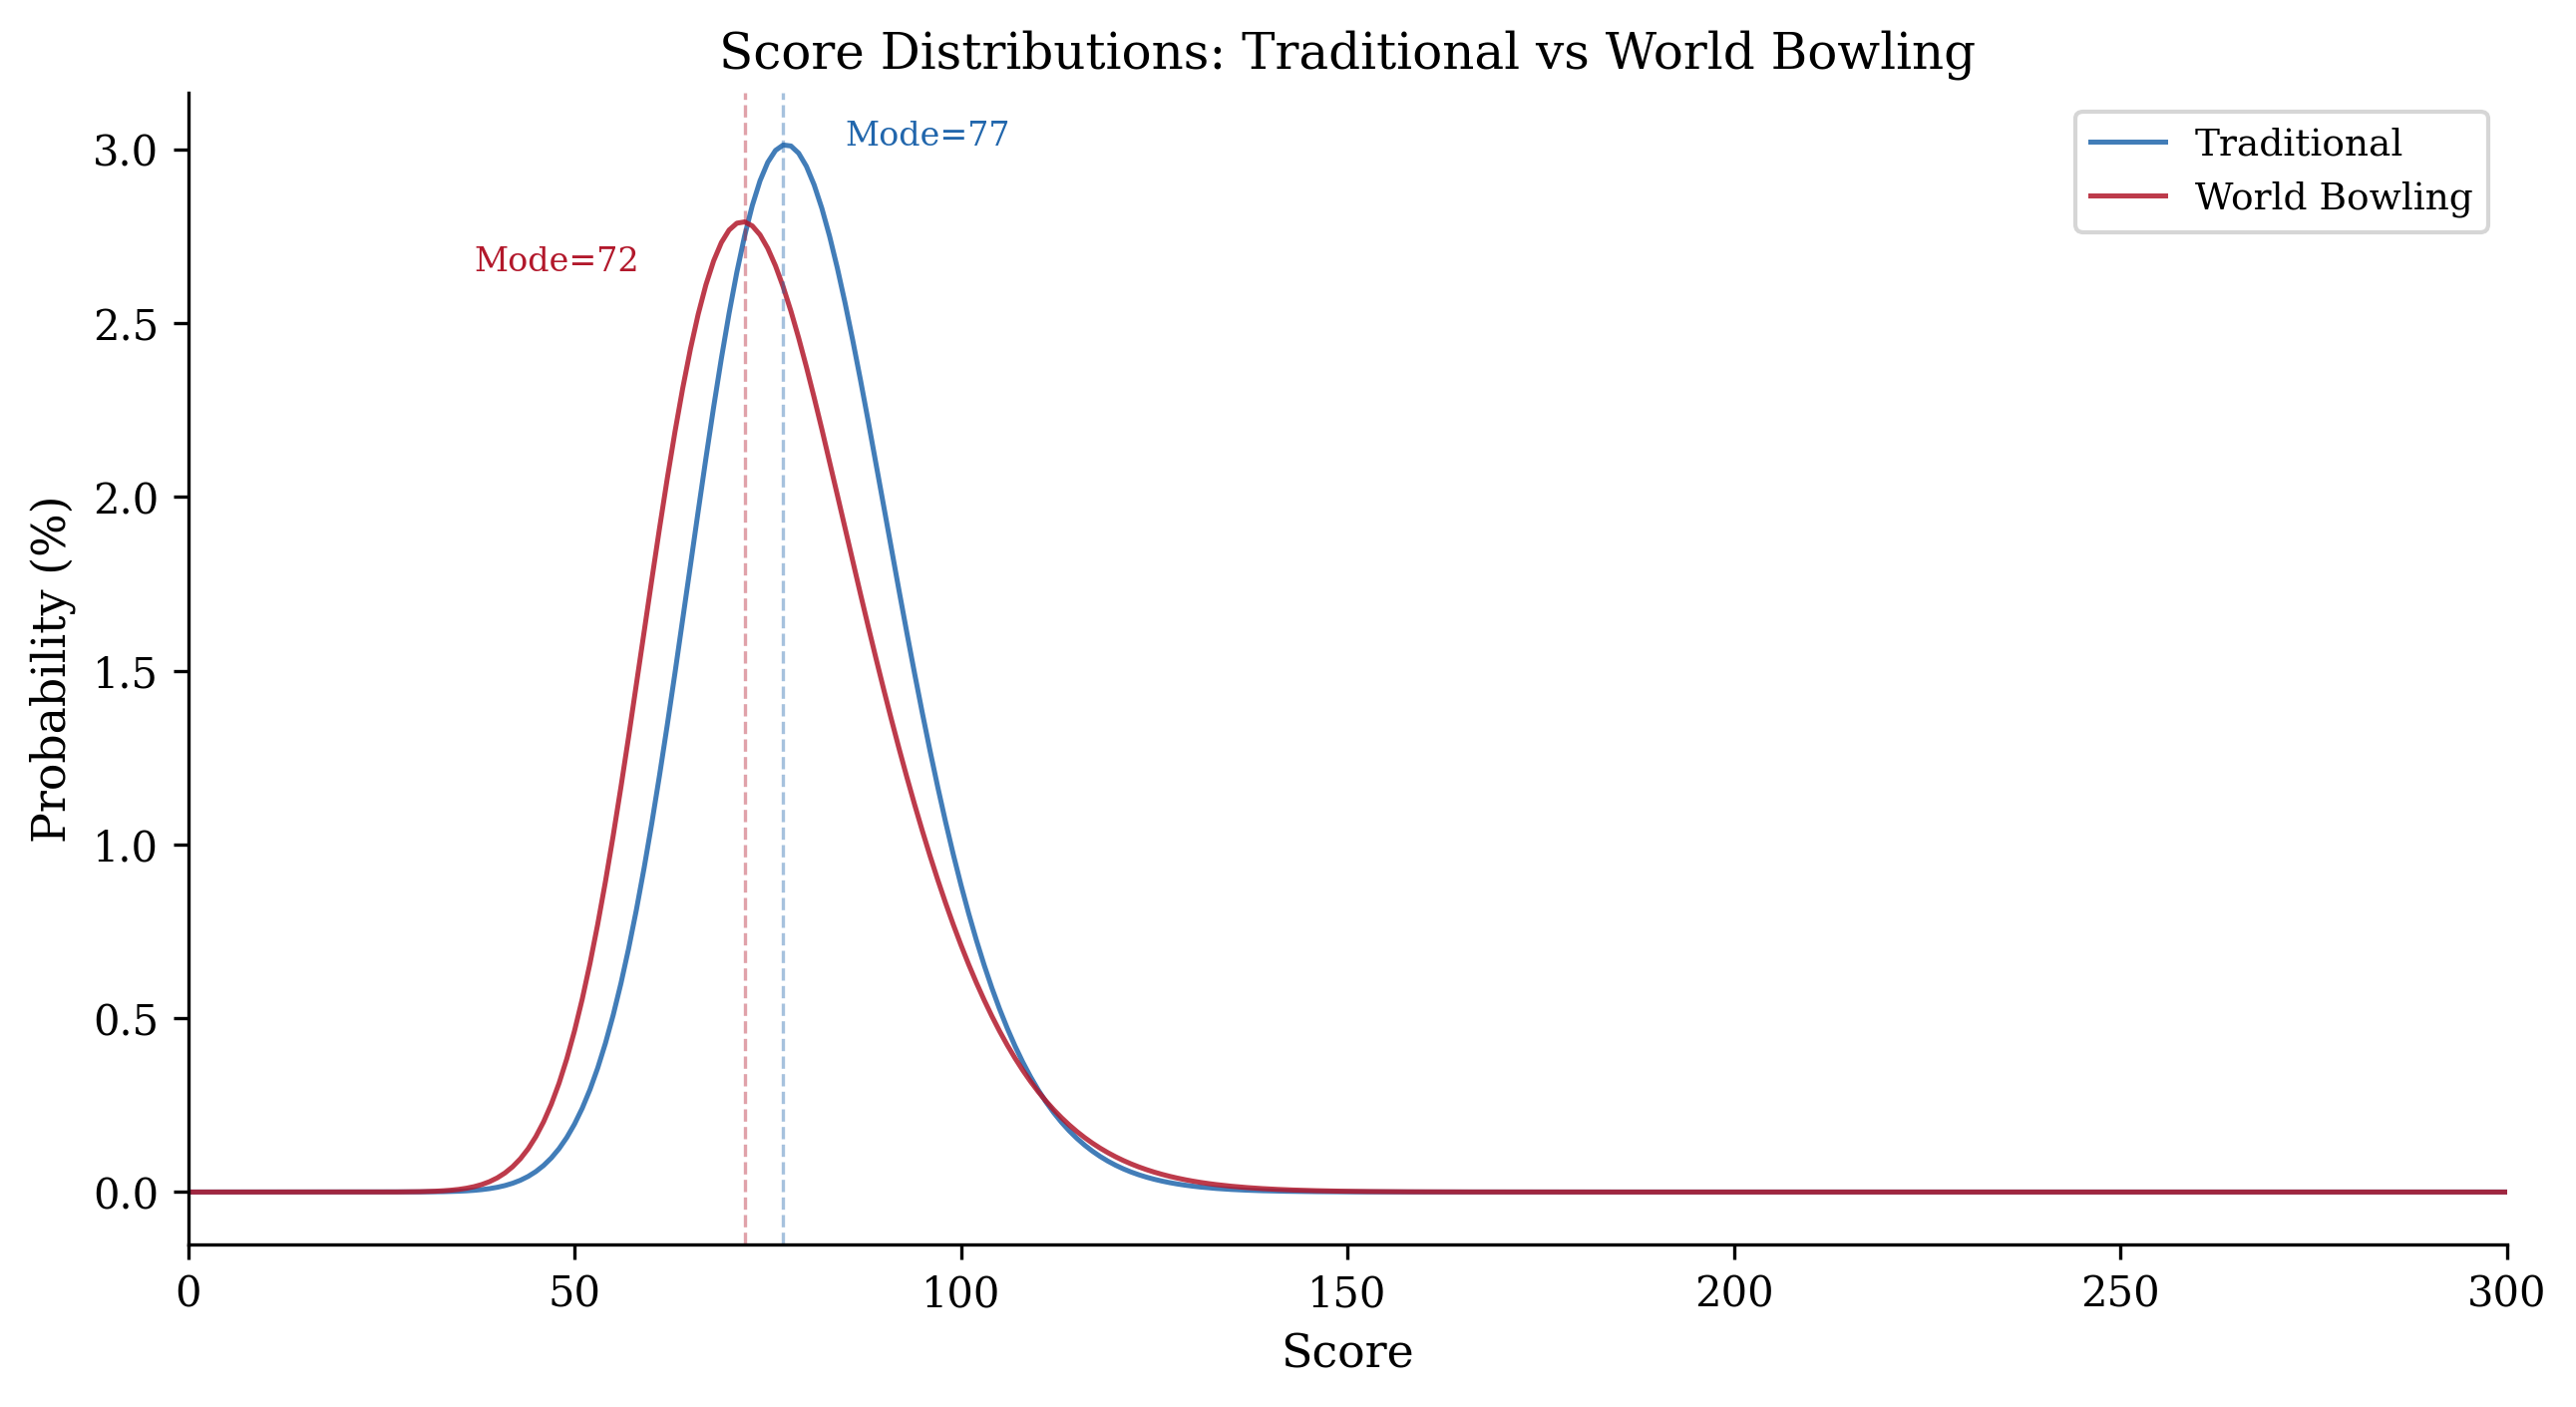
\includegraphics[width=1\linewidth,height=\textheight,keepaspectratio]{../figures/fig1_distribution_overlay.png}

}

\caption{\label{fig-distribution}Score distributions under traditional
and World Bowling scoring, computed by exact combinatorial enumeration
over all possible games. Dashed lines indicate modes.}

\end{figure}%

\subsection{Impossible Scores}\label{impossible-scores}

A structural property of World Bowling scoring is the impossibility of
scores in the range 290--299. This arises because 9 strikes yield at
most \(9 \times 30 + 19 = 289\) (9 strikes plus one maximum spare of 10
+ 9), while 10 strikes yield exactly 300. No sequence of legal balls can
produce a game score between 290 and 299 inclusive under World Bowling
rules. This gap is not a curiosity; it is a direct consequence of the
linear, frame-independent scoring structure, and it reveals a
fundamental property: \textbf{the score space is not fully utilised}.

\begin{figure}[htbp]

\centering{

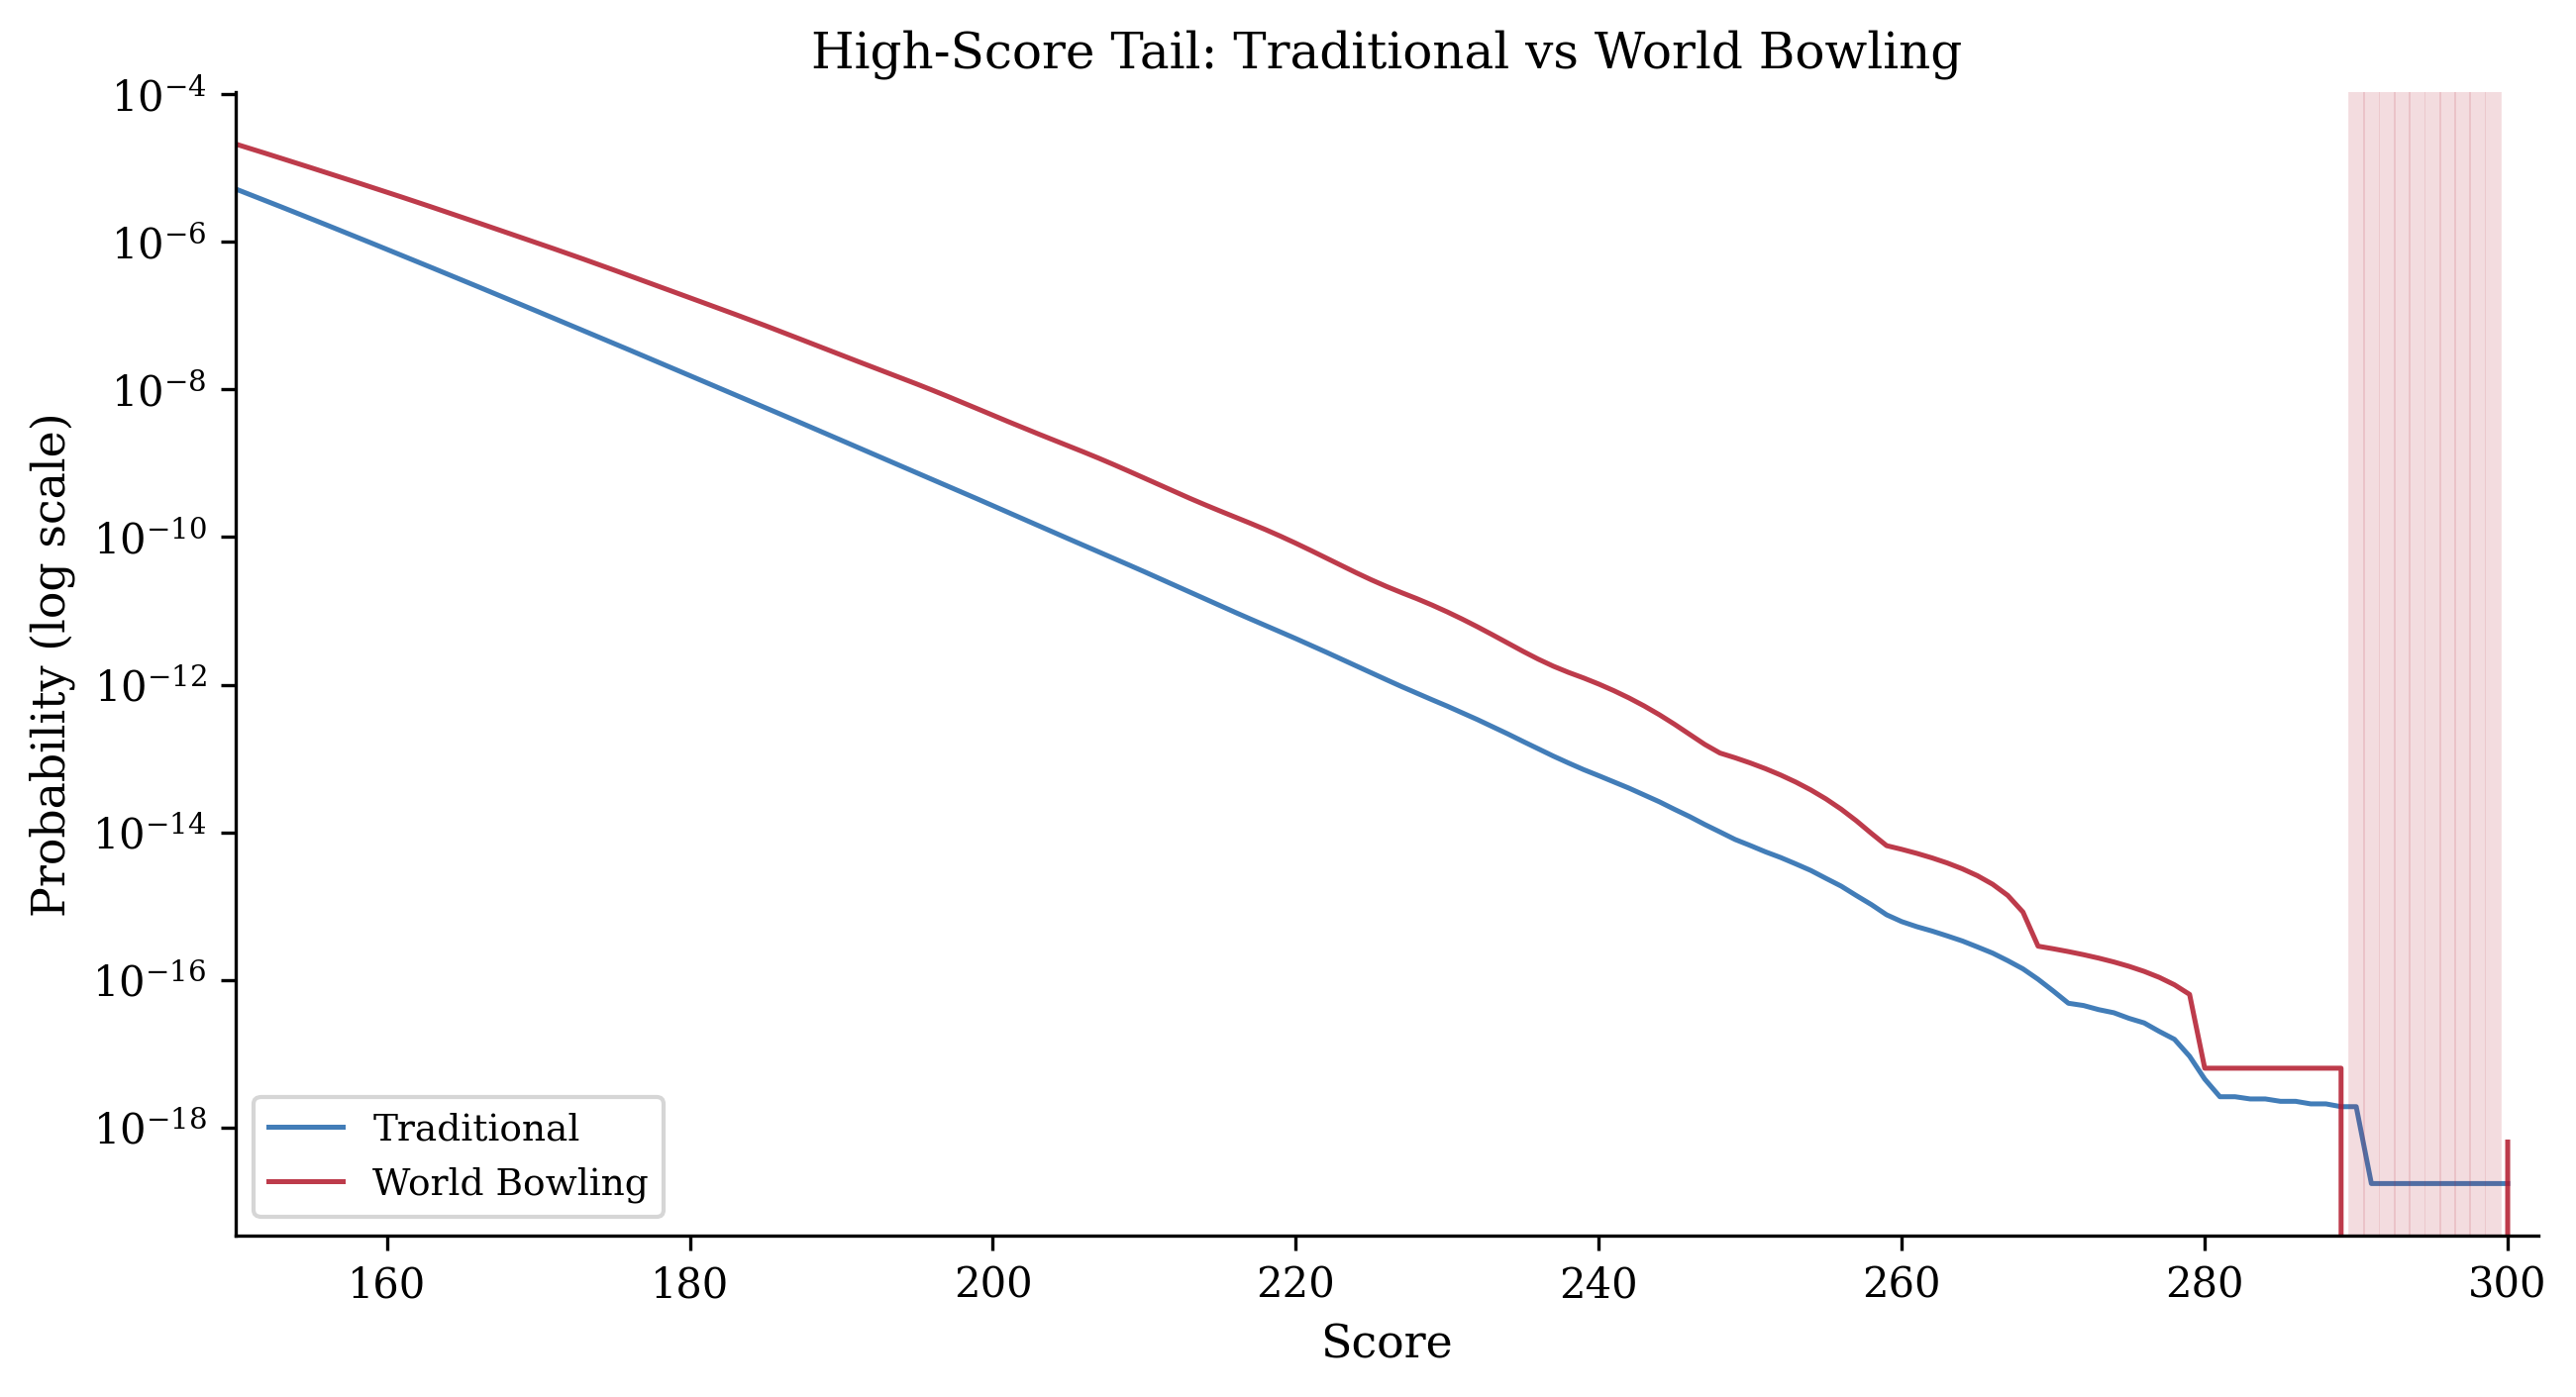
\includegraphics[width=1\linewidth,height=\textheight,keepaspectratio]{../figures/fig2_high_score_tail.png}

}

\caption{\label{fig-tail}High-score tail on log scale. The shaded region
at 290--299 marks scores that are mathematically impossible under World
Bowling.}

\end{figure}%

\subsection{High-Score Compression}\label{high-score-compression}

The number of distinct game sequences producing each high score differs
markedly between systems:

\begin{longtable}[]{@{}lll@{}}
\caption{Number of distinct game sequences producing each high
score.}\label{tbl-compression}\tabularnewline
\toprule\noalign{}
Score & Traditional & World Bowling \\
\midrule\noalign{}
\endfirsthead
\toprule\noalign{}
Score & Traditional & World Bowling \\
\midrule\noalign{}
\endhead
\bottomrule\noalign{}
\endlastfoot
200 & 1,526,313,637 & 7,019,752,752 \\
240 & 335,065 & 1,599,447 \\
260 & 3,534 & 9,225 \\
280 & 26 & 10 \\
290 & 11 & 0 (impossible) \\
300 & 1 & 1 \\
\end{longtable}

At scores of 200 and above, World Bowling consistently offers more paths
to the same score. This score compression means the score scale is
coarser at the top: more distinct games collapse onto the same number,
leaving fewer available values to separate high-scoring performances.
Whether a coarser scale also reduces the system's ability to
discriminate \emph{player skill}, as opposed to merely separating
individual games, is a separate question that the raw counts here cannot
settle; we address it directly with a signal-to-noise reliability
analysis in Part 2.

\section{Sequence Sensitivity}\label{sequence-sensitivity}

\subsection{Commutativity of World Bowling
Scoring}\label{commutativity-of-world-bowling-scoring}

\textbf{Proposition 1.} \emph{Under World Bowling scoring, the total
game score is invariant under any permutation of the ten frames.}

\emph{Proof.} Let \(f_i\) denote the score of frame \(i\) under World
Bowling rules. The total game score is \(S = \sum_{i=1}^{10} f_i\).
Since each \(f_i\) is computed from balls thrown within frame \(i\)
alone, and addition is commutative and associative, any permutation
\(\sigma\) of the frames yields
\(S' = \sum_{i=1}^{10} f_{\sigma(i)} = S\). \(\square\)

The proposition is deliberately elementary: the proof is commutativity
of addition, and no deeper machinery is needed. We state it formally
because it is the structural anchor for everything that follows. The
contribution of this paper is not the proof itself but the
quantification, in Part 2, of exactly what a scoring system gives up by
having this property.

This property, commutativity with respect to frame order, does not hold
for traditional scoring. Under traditional scoring, a strike in frame
\(i\) depends on balls thrown in frames \(i+1\) and potentially \(i+2\).
Reordering frames changes which balls serve as bonuses, and therefore
changes the score.

\subsection{Empirical Demonstration}\label{empirical-demonstration}

We compute scores for fixed frame compositions under varying orderings.
Consider 9 frames comprising 5 strikes and 4 spares (5,5) in various
orderings, followed by a neutral frame 10 (5, 4):

\begin{longtable}[]{@{}lll@{}}
\caption{Scores for four orderings of the same frame composition (5
strikes + 4 spares).}\label{tbl-sequence}\tabularnewline
\toprule\noalign{}
Sequence (9 frames + neutral 10th) & Traditional & World Bowling \\
\midrule\noalign{}
\endfirsthead
\toprule\noalign{}
Sequence (9 frames + neutral 10th) & Traditional & World Bowling \\
\midrule\noalign{}
\endhead
\bottomrule\noalign{}
\endlastfoot
5 strikes then 4 spares & 204 & 219 \\
Alternating: strike, spare × 4, strike & 188 & 219 \\
4 spares then 5 strikes & 208 & 219 \\
X, sp, sp, X, sp, X, X, sp, X & 188 & 219 \\
\end{longtable}

Under World Bowling, all four orderings score identically (219). Under
traditional scoring, the score varies by 20 points (188--208) depending
solely on the ordering.

\begin{figure}[htbp]

\centering{

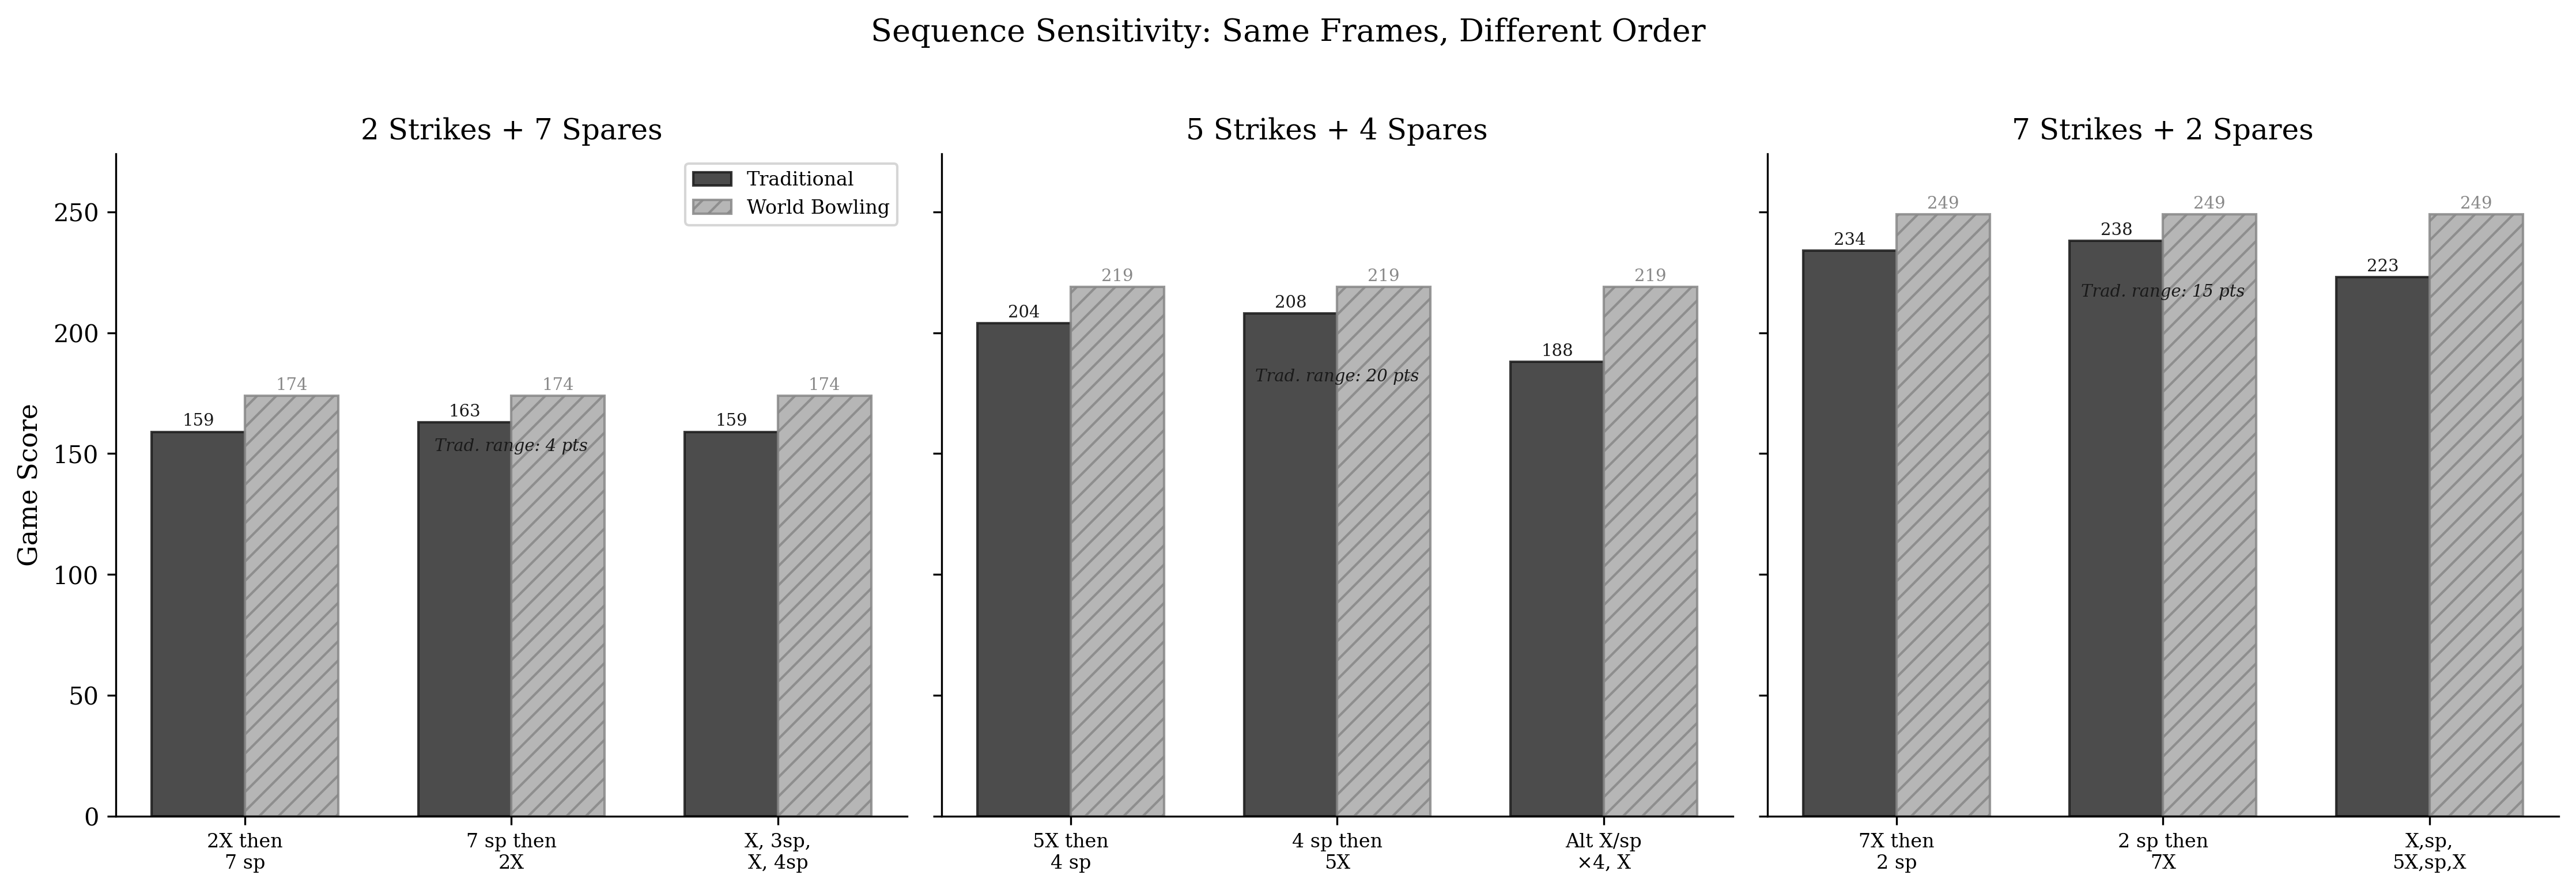
\includegraphics[width=1\linewidth,height=\textheight,keepaspectratio]{../figures/fig5_sequence_sensitivity.png}

}

\caption{\label{fig-sequence}Sequence sensitivity across three
compositions (2, 5, and 7 strikes out of 9 frames). In each panel, the
same frames are reordered. World Bowling scores are identical for all
orderings; traditional scores vary, with the range increasing at higher
strike counts.}

\end{figure}%

\subsection{Exhaustive Permutation
Analysis}\label{exhaustive-permutation-analysis}

To quantify the full extent of sequence sensitivity, we enumerate all
distinct permutations of fixed frame compositions and compute the score
under each system. For compositions of \(k\) strikes and \((9-k)\)
spares in frames 1--9:

\begin{longtable}[]{@{}lllll@{}}
\caption{Exhaustive permutation analysis. Traditional score range and
standard deviation grow with the mix of frame types; World Bowling range
is exactly zero for every
composition.}\label{tbl-permutations}\tabularnewline
\toprule\noalign{}
Composition & Orderings & Trad. range & Trad. SD & WB range \\
\midrule\noalign{}
\endfirsthead
\toprule\noalign{}
Composition & Orderings & Trad. range & Trad. SD & WB range \\
\midrule\noalign{}
\endhead
\bottomrule\noalign{}
\endlastfoot
1 strike + 8 spares & 9 & 5 & 1.7 & 0 \\
2 strikes + 7 spares & 36 & 6 & 2.1 & 0 \\
3 strikes + 6 spares & 84 & 11 & 2.9 & 0 \\
4 strikes + 5 spares & 126 & 16 & 4.2 & 0 \\
5 strikes + 4 spares & 126 & 21 & 5.5 & 0 \\
6 strikes + 3 spares & 84 & 26 & 6.4 & 0 \\
7 strikes + 2 spares & 36 & 26 & 6.6 & 0 \\
8 strikes + 1 spare & 9 & 15 & 5.6 & 0 \\
\end{longtable}

The World Bowling score range is exactly zero for every composition,
confirming Proposition 1 empirically. The traditional score range grows
with the mix of frame types, peaking at 26 points for compositions with
6--7 strikes. When open frames are included alongside strikes, the range
increases further: 5 strikes mixed with 4 open frames (5, 4) produces a
39-point range across 126 orderings.

\begin{figure}[htbp]

\centering{

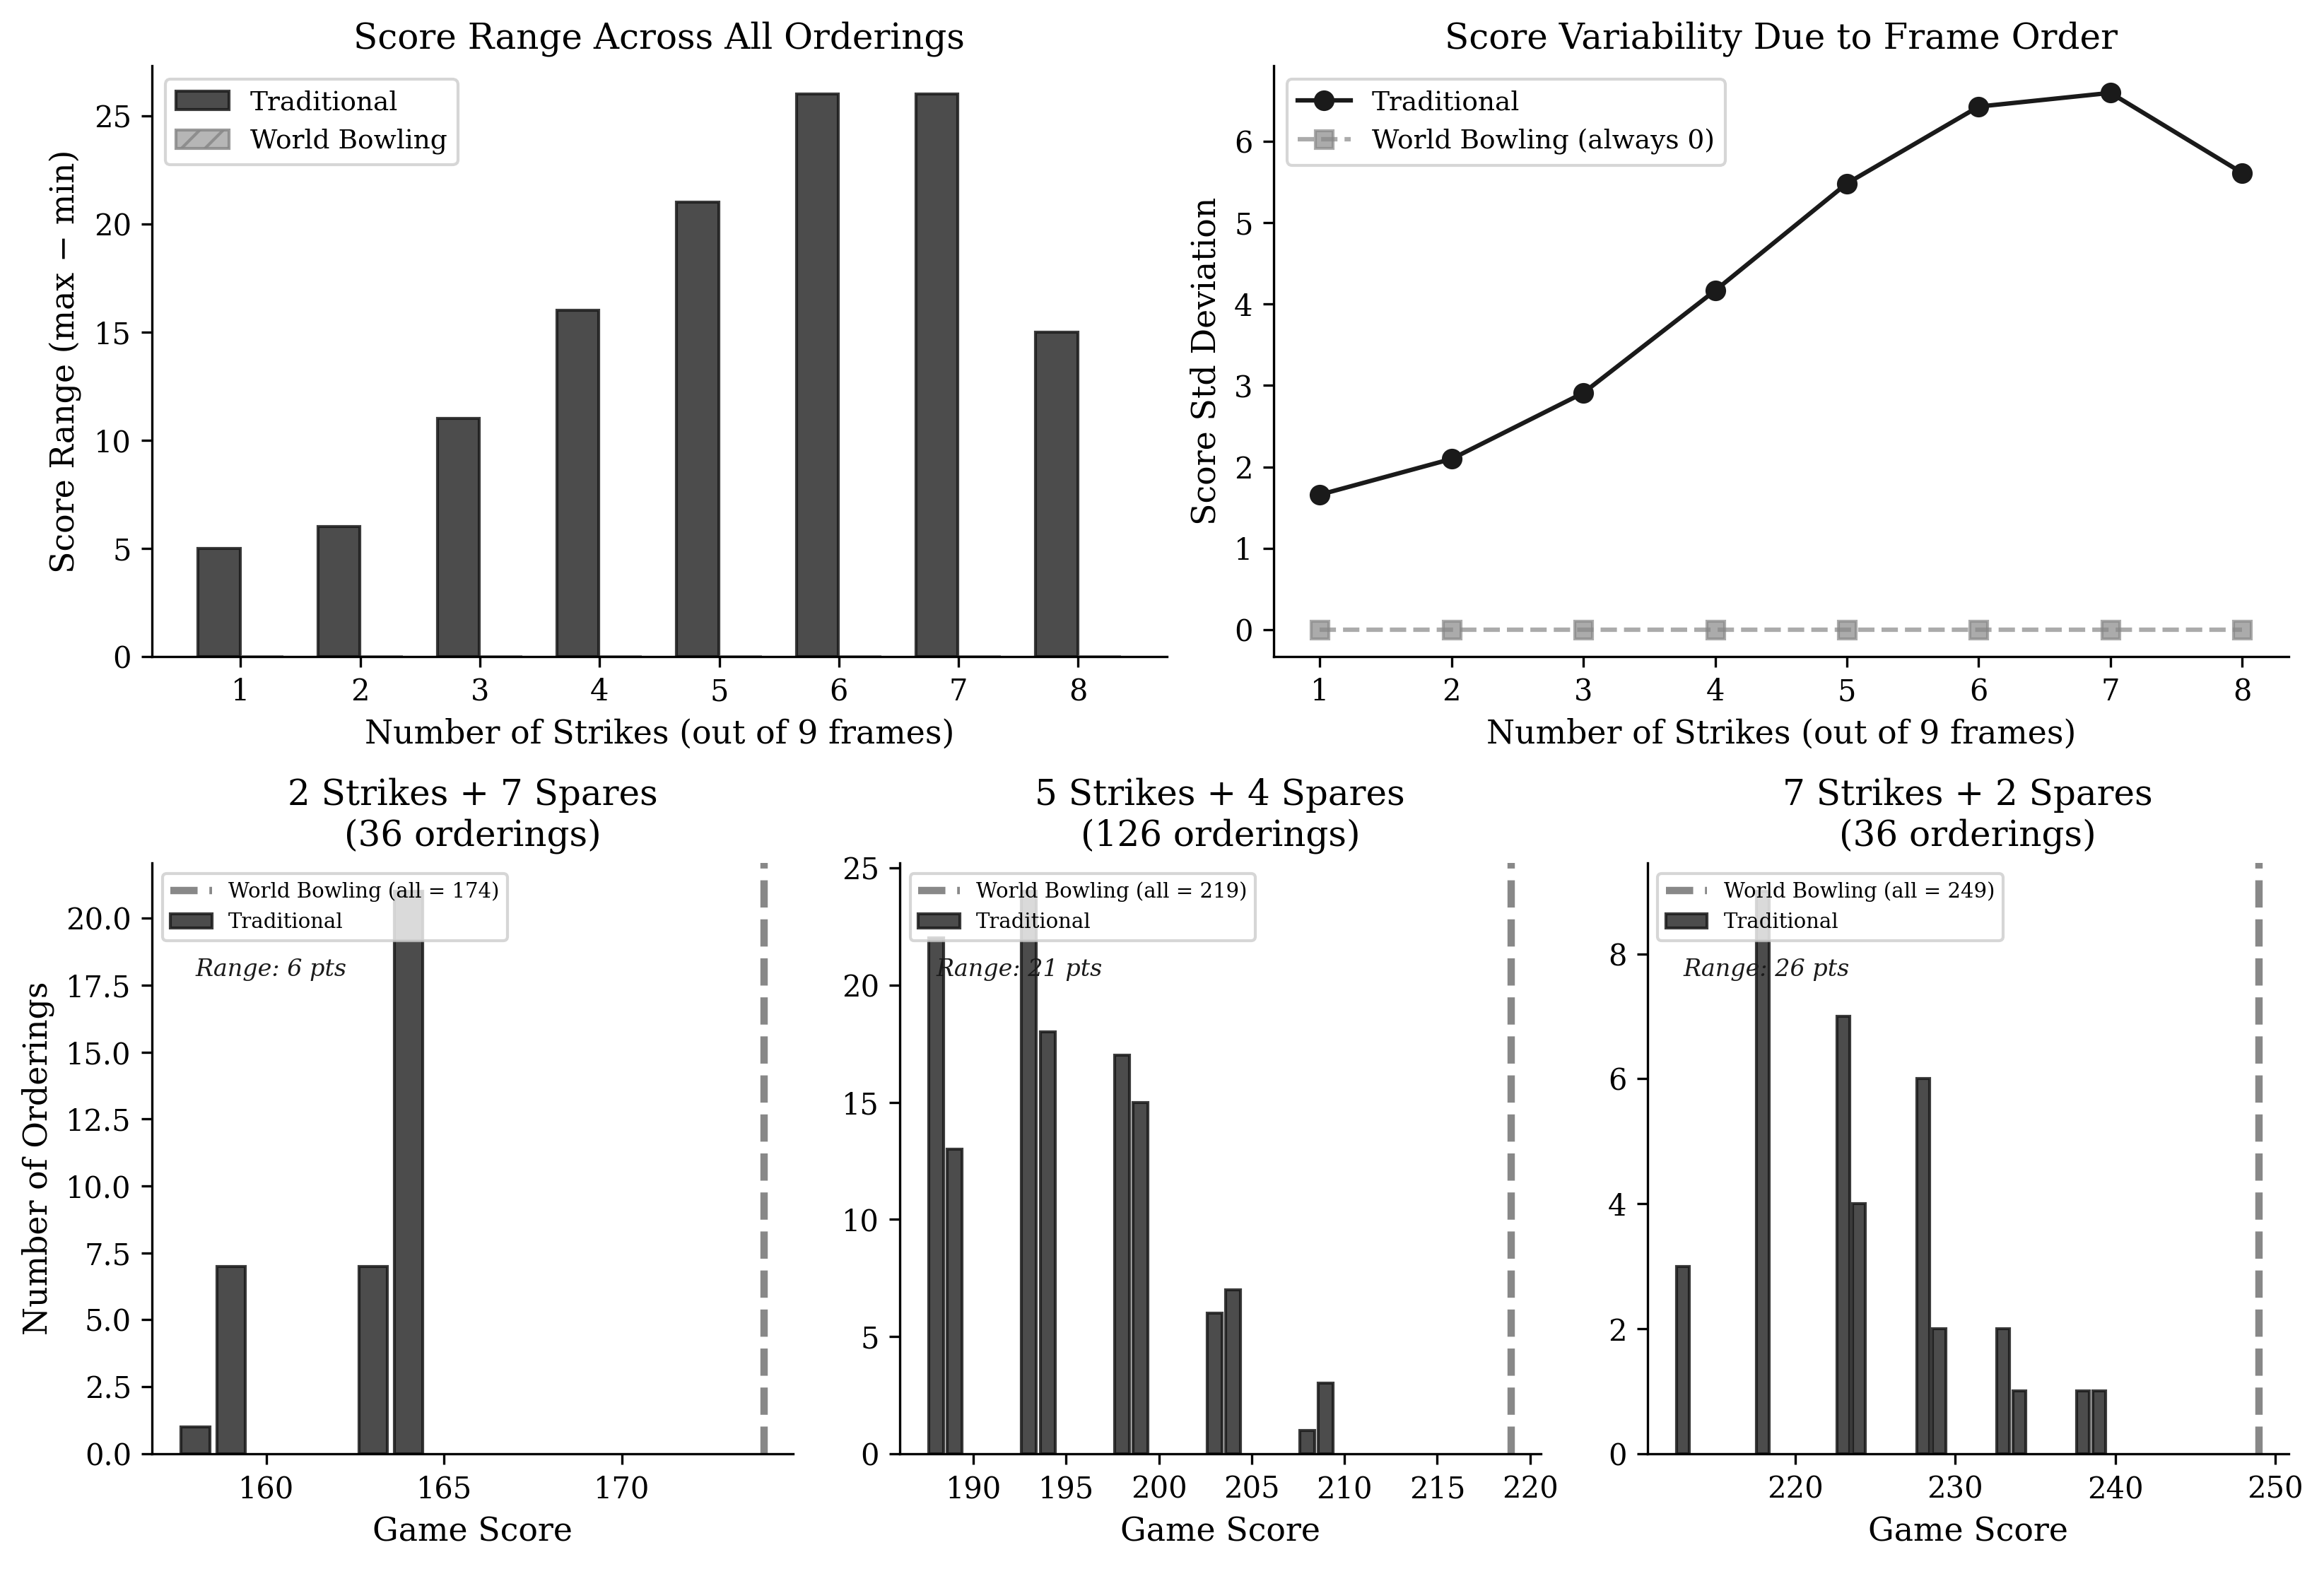
\includegraphics[width=1\linewidth,height=\textheight,keepaspectratio]{../figures/fig6_permutation_analysis.png}

}

\caption{\label{fig-permutation}Sequence sensitivity of fixed frame
compositions. Top: score range and score standard deviation across all
orderings, by composition. Bottom: score distribution across all
orderings for three compositions (2, 5, and 7 strikes). Traditional
scores spread across a range that widens with strike count; World
Bowling is exactly zero throughout and collapses to a single value
(dashed line).}

\end{figure}%

\subsection{Implications for Skill}\label{implications-for-skill}

Sequence sensitivity has a direct sporting interpretation. In
competitive bowling, a player who strings consecutive strikes together
is demonstrating a qualitatively different level of performance than one
who scatters the same number of strikes throughout a game. The
traditional scoring system encodes this distinction numerically. The
World Bowling system does not.

The maximum score achievable with a fixed number of strikes is higher
when those strikes are consecutive (due to compounding bonuses from
subsequent strikes), creating a score incentive for sustained
excellence. Under World Bowling, a bowler who throws five consecutive
strikes in frames 1--5 and then opens all remaining frames achieves the
same score as one who alternates strikes and open frames, regardless of
how much more difficult the sustained streak was to achieve.

\section{The Reward Gradient for Consecutive
Strikes}\label{the-reward-gradient-for-consecutive-strikes}

We define the \textbf{marginal strike value} as the increase in game
score when one additional open frame (5, 4) is replaced by a strike, all
other frames remaining constant. Under World Bowling this value is
trivially constant: \(30 - 9 = 21\) points per strike added.

Under traditional scoring, the marginal value depends on the surrounding
context:

\begin{longtable}[]{@{}
  >{\raggedright\arraybackslash}p{(\linewidth - 8\tabcolsep) * \real{0.2000}}
  >{\raggedright\arraybackslash}p{(\linewidth - 8\tabcolsep) * \real{0.2000}}
  >{\raggedright\arraybackslash}p{(\linewidth - 8\tabcolsep) * \real{0.2000}}
  >{\raggedright\arraybackslash}p{(\linewidth - 8\tabcolsep) * \real{0.2000}}
  >{\raggedright\arraybackslash}p{(\linewidth - 8\tabcolsep) * \real{0.2000}}@{}}
\caption{Marginal value of each additional consecutive
strike.}\label{tbl-gradient}\tabularnewline
\toprule\noalign{}
\begin{minipage}[b]{\linewidth}\raggedright
Consecutive strikes
\end{minipage} & \begin{minipage}[b]{\linewidth}\raggedright
Trad. Score
\end{minipage} & \begin{minipage}[b]{\linewidth}\raggedright
World Score
\end{minipage} & \begin{minipage}[b]{\linewidth}\raggedright
Trad. Marginal
\end{minipage} & \begin{minipage}[b]{\linewidth}\raggedright
World Marginal
\end{minipage} \\
\midrule\noalign{}
\endfirsthead
\toprule\noalign{}
\begin{minipage}[b]{\linewidth}\raggedright
Consecutive strikes
\end{minipage} & \begin{minipage}[b]{\linewidth}\raggedright
Trad. Score
\end{minipage} & \begin{minipage}[b]{\linewidth}\raggedright
World Score
\end{minipage} & \begin{minipage}[b]{\linewidth}\raggedright
Trad. Marginal
\end{minipage} & \begin{minipage}[b]{\linewidth}\raggedright
World Marginal
\end{minipage} \\
\midrule\noalign{}
\endhead
\bottomrule\noalign{}
\endlastfoot
0 & 90 & 90 & n/a & n/a \\
1 & 100 & 111 & +10 & +21 \\
2 & 116 & 132 & +16 & +21 \\
3 & 137 & 153 & +21 & +21 \\
4 & 158 & 174 & +21 & +21 \\
5 & 179 & 195 & +21 & +21 \\
10 & 300 & 300 & +37 & +21 \\
\end{longtable}

Two observations are immediate. First, the initial strikes are
undervalued in traditional scoring relative to World Bowling: the first
strike adds only 10 points compared to 21 under World Bowling. This is
because the bonus from a lone strike depends on subsequent balls that
are in this model open frames (5, 4 = 9 pins), capping the bonus at 9.
Second, the final strike in a perfect game is worth 37 points under
traditional scoring, substantially more than World Bowling's flat 21,
because it is preceded by two strikes that each earn its bonus
retroactively.

This structure rewards the \emph{completion} of a skill streak more than
its initiation. The first strike of a sequence is worth relatively
little; the strike that extends a string is worth substantially more.
Under World Bowling, every strike is worth exactly the same regardless
of what surrounds it.

\begin{figure}[htbp]

\centering{

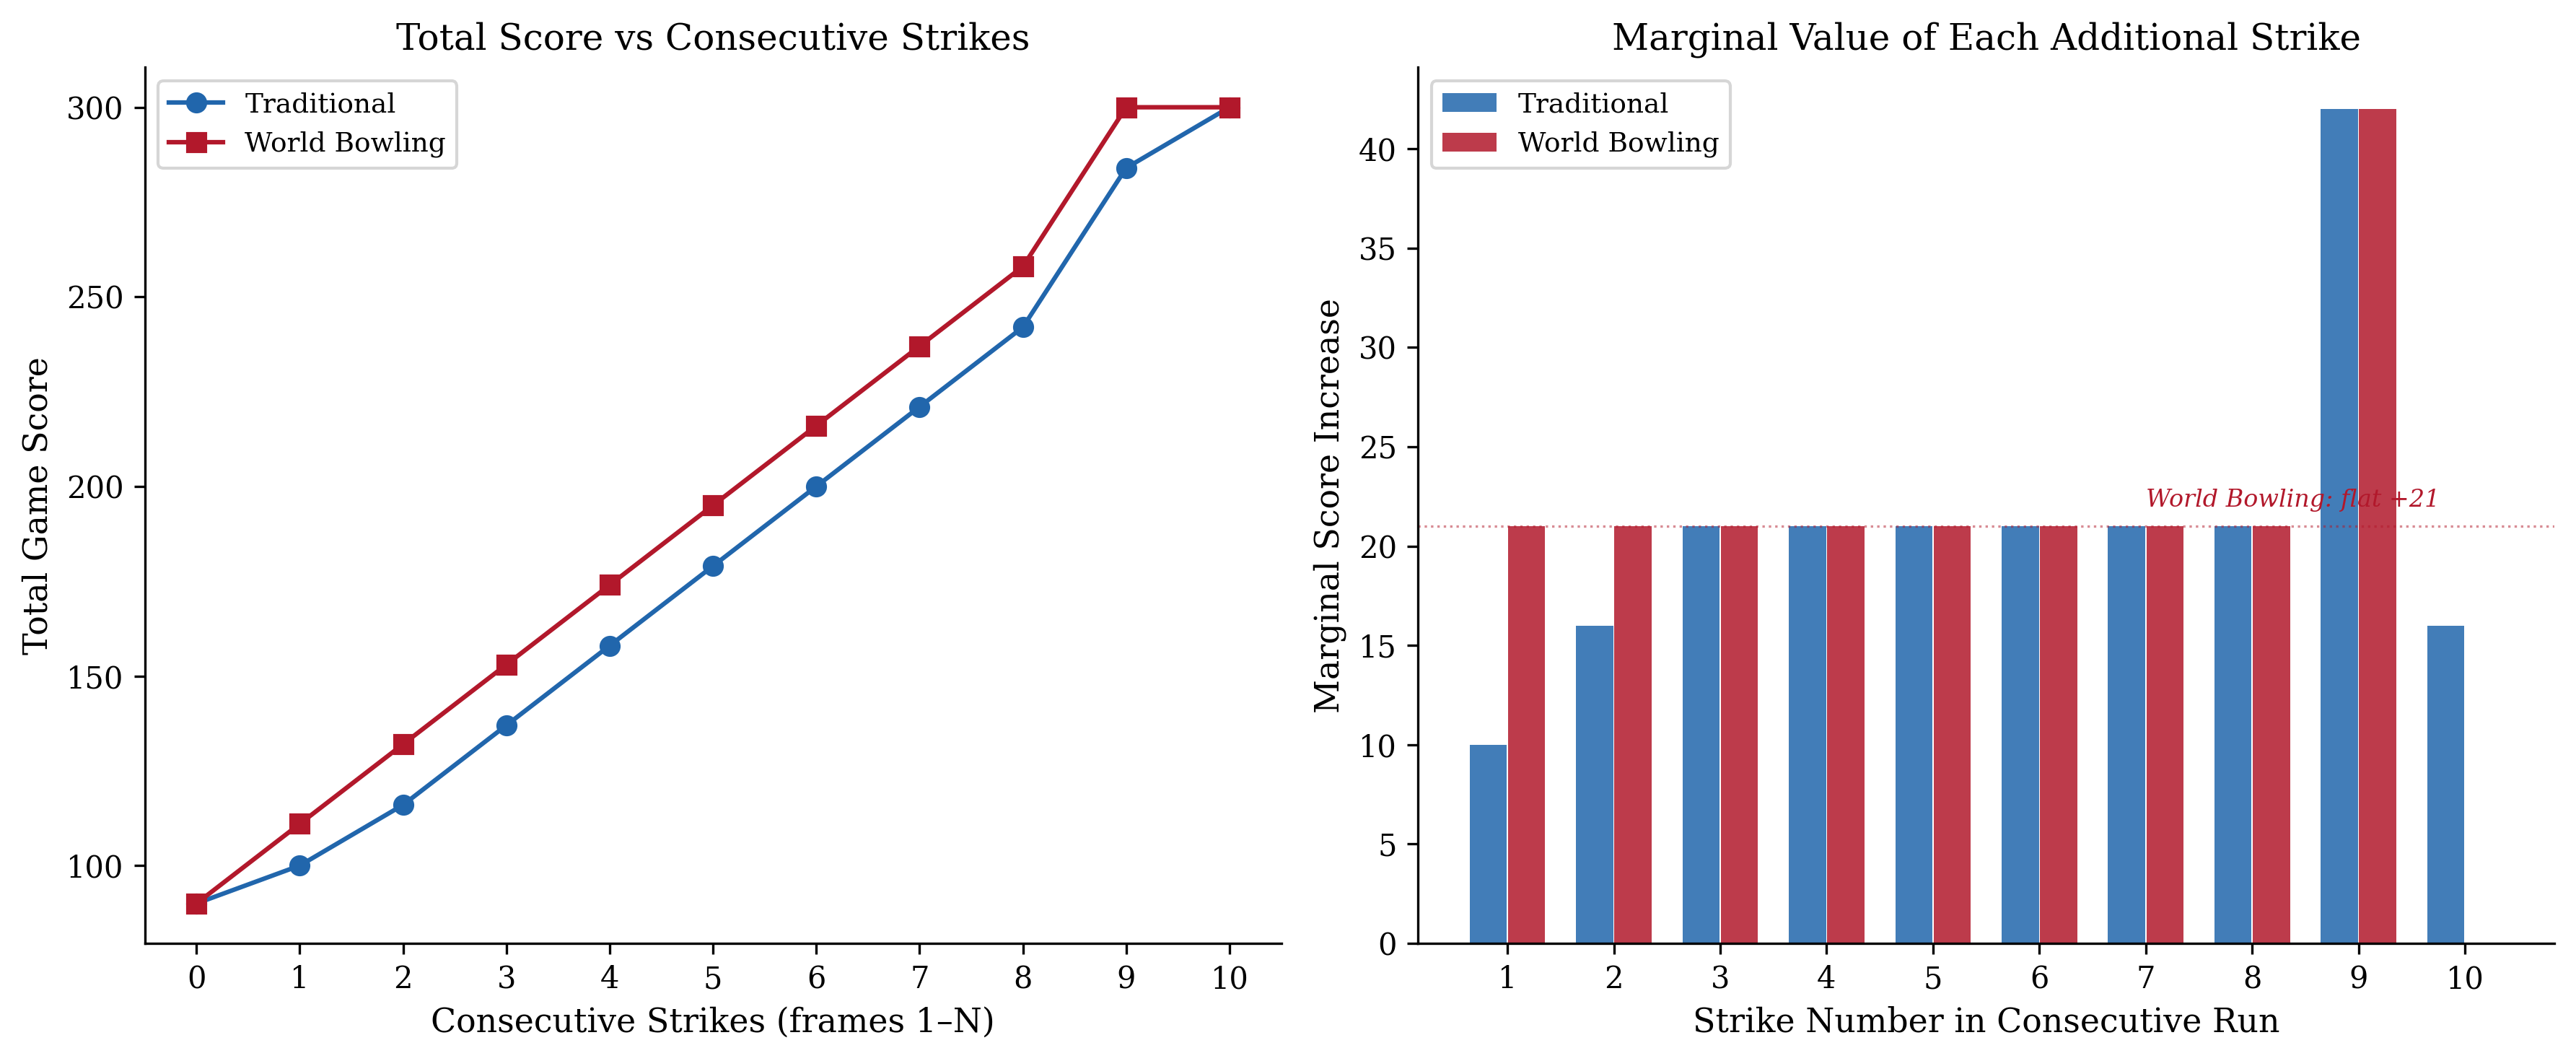
\includegraphics[width=1\linewidth,height=\textheight,keepaspectratio]{../figures/fig3_reward_gradient.png}

}

\caption{\label{fig-gradient}Marginal value of each additional
consecutive strike, shown for three different non-strike fill patterns:
weak (3,2), mid (5,4), and strong (8,1). The compounding pattern in
traditional scoring and the flat World Bowling marginal are structural,
not dependent on the fill choice.}

\end{figure}%

\section*{Part 2: Skill-Weighted
Simulation}\label{part-2-skill-weighted-simulation}
\addcontentsline{toc}{section}{Part 2: Skill-Weighted Simulation}

\section{Simulation Model}\label{simulation-model}

\subsection{Player Model}\label{player-model}

To ground the mathematical analysis in realistic playing conditions, we
simulate bowling games across six empirically motivated skill tiers.
Each player is characterised by three parameters: strike probability
(\(p_s\)), spare conversion probability (\(p_{sp}\)), and mean
first-ball pin count when not striking. Tier parameters were calibrated
against published data from multiple sources: McCarthy
(\citeproc{ref-mccarthy2011}{2011}) reports a mean score of 205.65 (SD
31.91) across 278,579 PBA National Tour games, with individual bowler
ability estimates ranging from approximately 150 to 235; VanDerwerken \&
Kenter (\citeproc{ref-vanderwerken2018}{2018}) reports posterior mean
strike probabilities ranging from approximately 53\% to 66\% across 53
PBA bowlers; and USBC published league averages anchor the recreational
end.

\begin{longtable}[]{@{}lllll@{}}
\caption{Skill tier parameters. The recreational tier targets casual
bowlers based on USBC league averages. The professional tier targets the
PBA Tour season average of approximately 230, consistent with the upper
range of bowler ability estimates reported by McCarthy
(\citeproc{ref-mccarthy2011}{2011}). The Top 10 tier (73\% strike rate)
is extrapolated from the upper tail of the professional ability
distribution, representing the elite end of PBA performance
(\citeproc{ref-vanderwerken2018}{VanDerwerken \& Kenter, 2018};
\citeproc{ref-yaari2012}{Yaari \& Eisenmann,
2012}).}\label{tbl-tiers}\tabularnewline
\toprule\noalign{}
Skill Tier & Strike Rate & Spare Rate & Pin Mean & Target Trad. Mean \\
\midrule\noalign{}
\endfirsthead
\toprule\noalign{}
Skill Tier & Strike Rate & Spare Rate & Pin Mean & Target Trad. Mean \\
\midrule\noalign{}
\endhead
\bottomrule\noalign{}
\endlastfoot
Recreational & 4\% & 27\% & 4.2 & \textasciitilde90 \\
Club & 20\% & 47\% & 5.5 & \textasciitilde130 \\
Competitive & 40\% & 64\% & 6.5 & \textasciitilde175 \\
Elite & 55\% & 77\% & 7.2 & \textasciitilde210 \\
Professional & 66\% & 86\% & 7.8 & \textasciitilde230 \\
Top 10 & 73\% & 92\% & 8.2 & \textasciitilde245 \\
\end{longtable}

\subsection{Simulation Protocol}\label{simulation-protocol}

We employ three progressively realistic simulation models to ensure
robustness of results:

\begin{enumerate}
\def\labelenumi{\arabic{enumi}.}
\item
  \textbf{Independent model (base case).} Each ball is generated
  independently: the first ball of each frame is a strike with
  probability \(p_s\), otherwise pins follow a binomial distribution;
  the second ball converts the spare with flat probability \(p_{sp}\).
\item
  \textbf{Momentum model.} Strike probability increases by 5 percentage
  points after a strike and decreases after an open frame, capturing the
  simplest form of sequential dependence.
\item
  \textbf{Markov chain model with spare difficulty.} Strike probability
  follows a first-order Markov chain with state-dependent transition
  probabilities informed by the empirical hot-hand magnitudes reported
  in VanDerwerken \& Kenter (\citeproc{ref-vanderwerken2018}{2018}), who
  built on the streak probability framework of Martin
  (\citeproc{ref-martin2006}{2006}) to fit 4th-order Markov models to
  26,102 PBA tournament games from 53 professional bowlers. Their
  posterior estimates show strike probability increasing by
  approximately 5--10 percentage points after consecutive strikes
  relative to a cold state. We apply conservative first-order transition
  ratios:
  \(P(\text{strike} \mid \text{prev. strike}) = p_s \times 1.15\),
  \(P(\text{strike} \mid \text{prev. spare}) = p_s \times 0.95\),
  \(P(\text{strike} \mid \text{prev. open}) = p_s \times 0.85\). Spare
  conversion is leave-dependent, with three difficulty classes
  consistent with the non-strike leave distributions reported in
  VanDerwerken \& Kenter (\citeproc{ref-vanderwerken2018}{2018}) Tables
  7--8: easy single-pin leaves (55\% of non-strike results, high
  conversion), moderate multi-pin leaves (35\%, baseline conversion),
  and splits (10\%, conversion rate reduced to 30\% of baseline).
\end{enumerate}

For each skill tier, we simulate 50,000 complete games under each model.
Every simulated game is scored under both traditional and World Bowling
rules, enabling paired comparison. The independent model provides a
conservative lower bound; the Markov model provides the most realistic
estimate.

\subsection{Tier Results}\label{tier-results}

\begin{longtable}[]{@{}lll@{}}
\caption{Simulated score statistics by skill tier (50,000 games
each).}\label{tbl-tierresults}\tabularnewline
\toprule\noalign{}
Skill Tier & Traditional Mean (SD) & World Bowling Mean (SD) \\
\midrule\noalign{}
\endfirsthead
\toprule\noalign{}
Skill Tier & Traditional Mean (SD) & World Bowling Mean (SD) \\
\midrule\noalign{}
\endhead
\bottomrule\noalign{}
\endlastfoot
Recreational & 91 (14.2) & 95 (17.7) \\
Club & 133 (21.2) & 149 (26.8) \\
Competitive & 176 (25.8) & 200 (28.1) \\
Elite & 209 (26.6) & 233 (25.1) \\
Professional & 232 (25.7) & 253 (21.4) \\
Top 10 & 246 (24.4) & 265 (18.6) \\
\end{longtable}

\begin{figure}[htbp]

\centering{

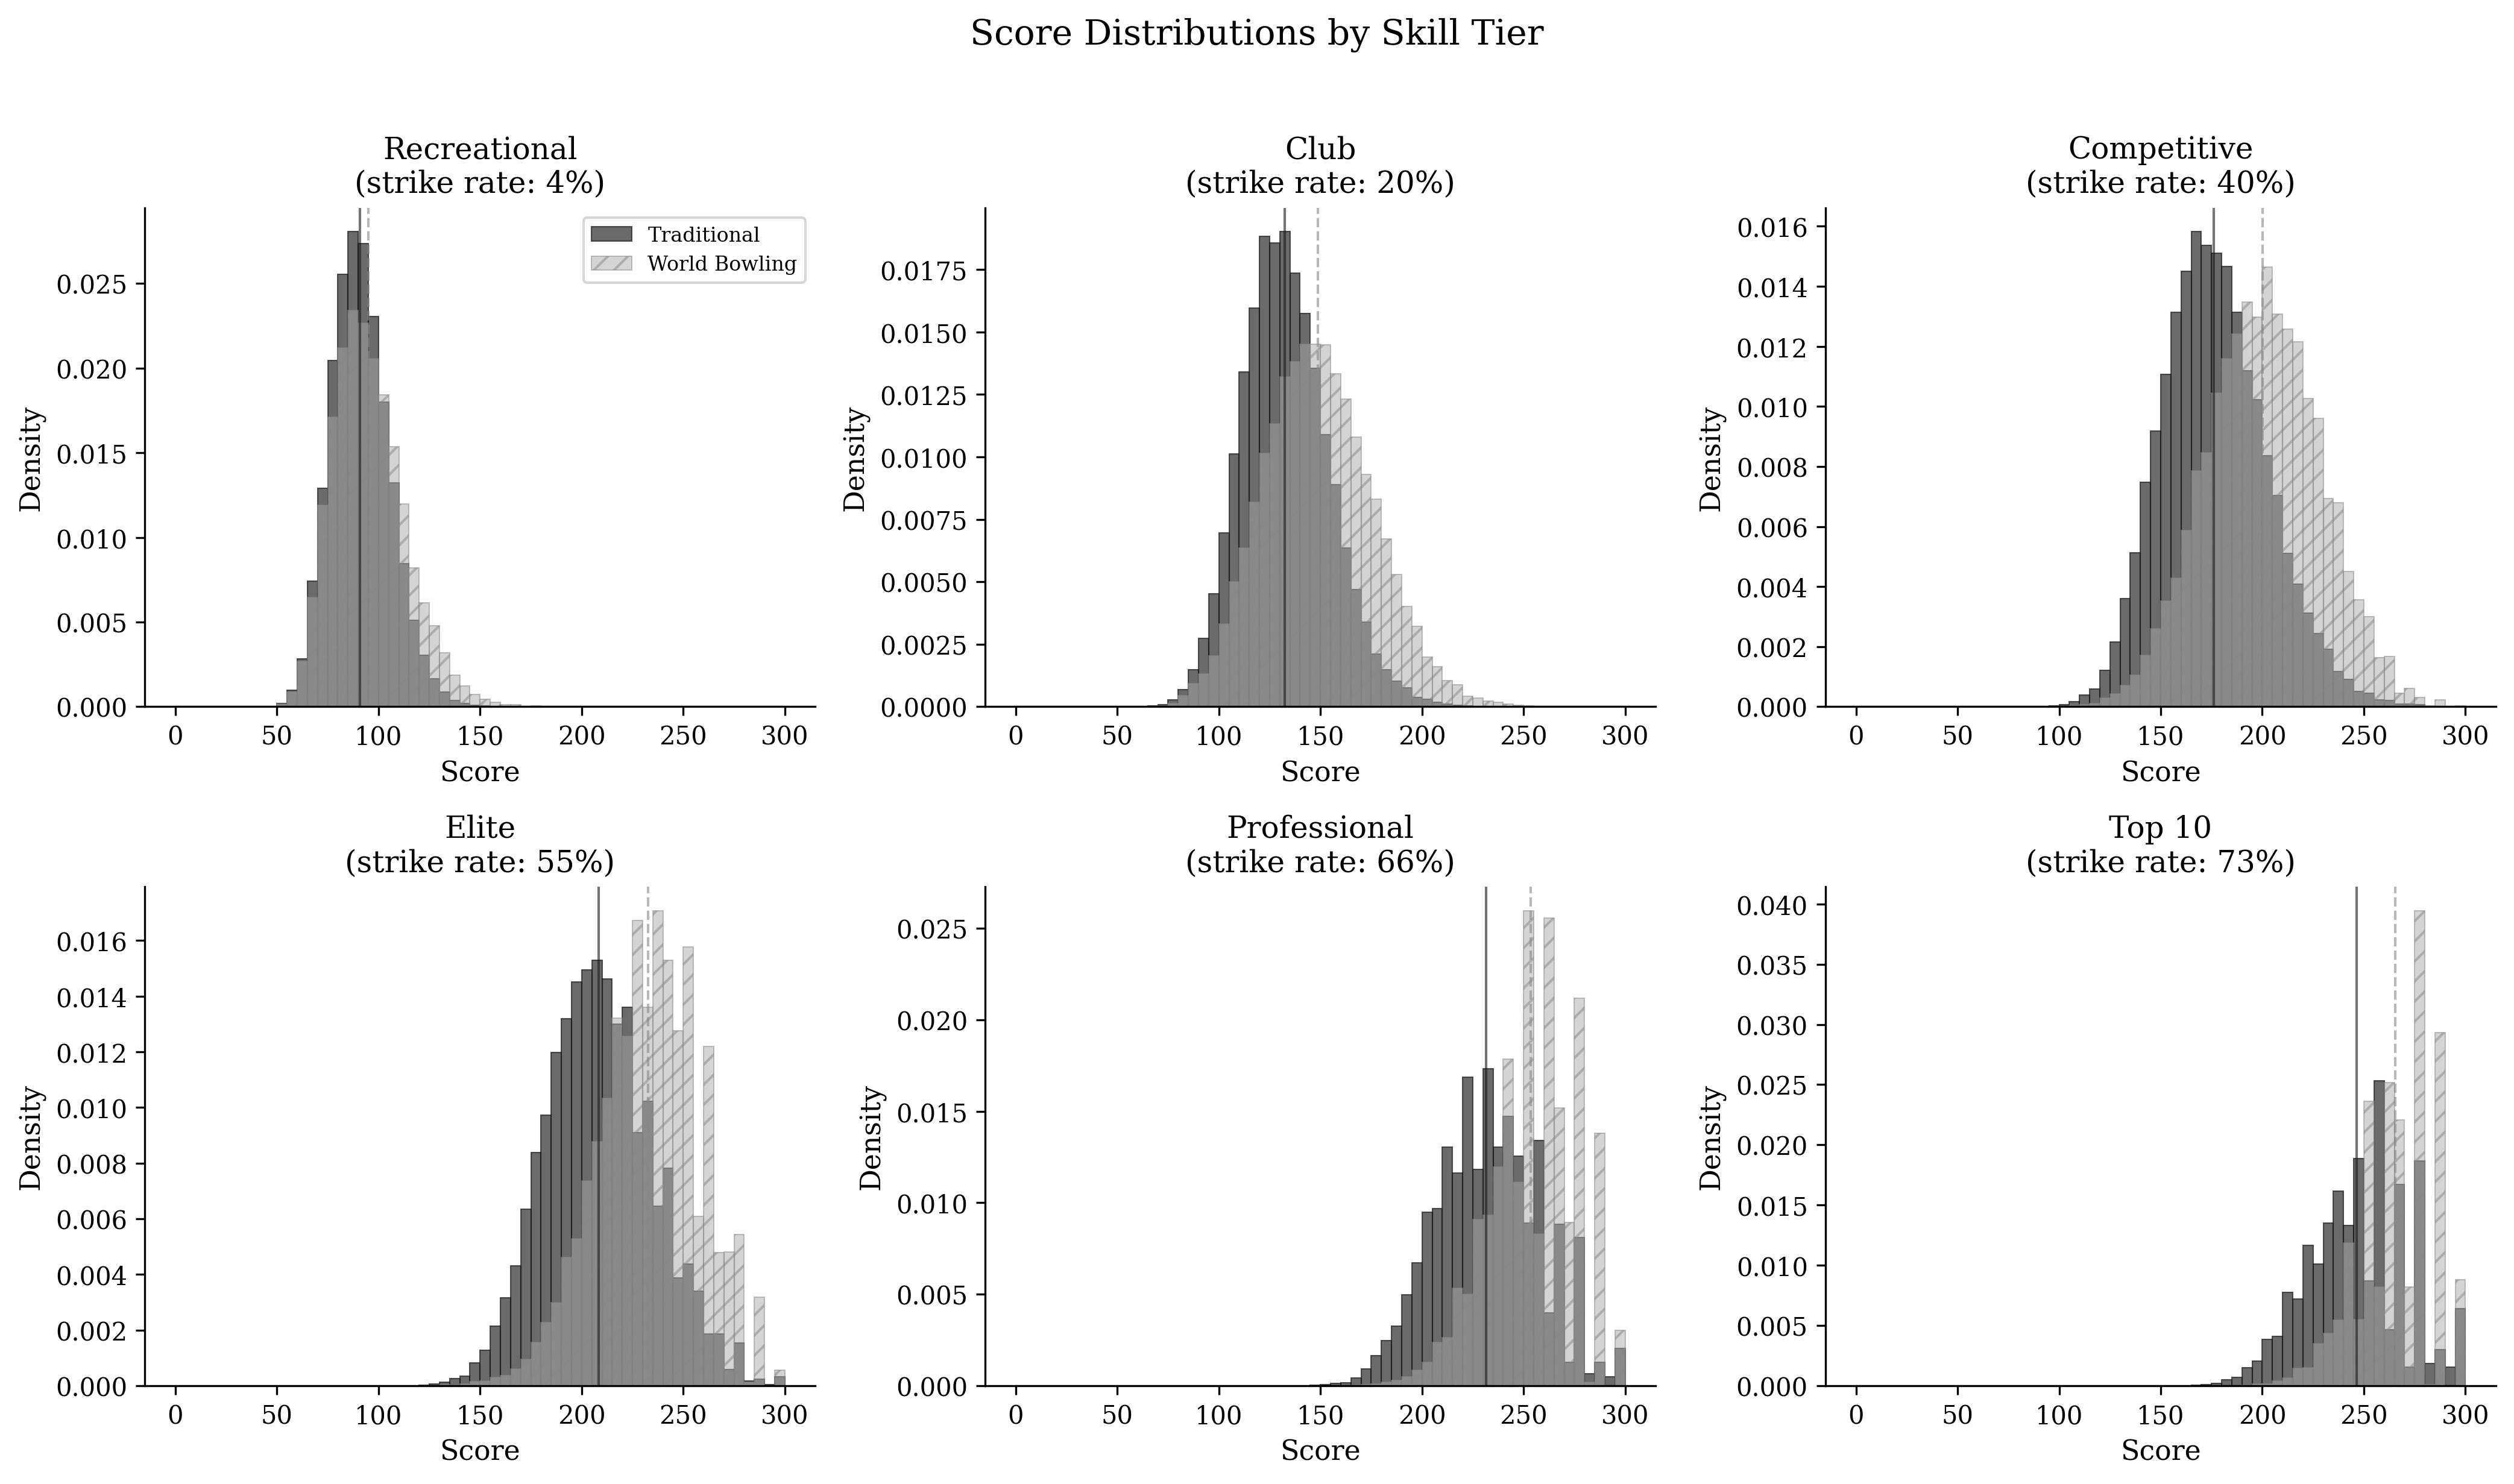
\includegraphics[width=1\linewidth,height=\textheight,keepaspectratio]{../figures/fig8_tier_distributions.png}

}

\caption{\label{fig-tierdist}Score distributions at each skill tier
under both scoring systems.}

\end{figure}%

\begin{figure}[htbp]

\centering{

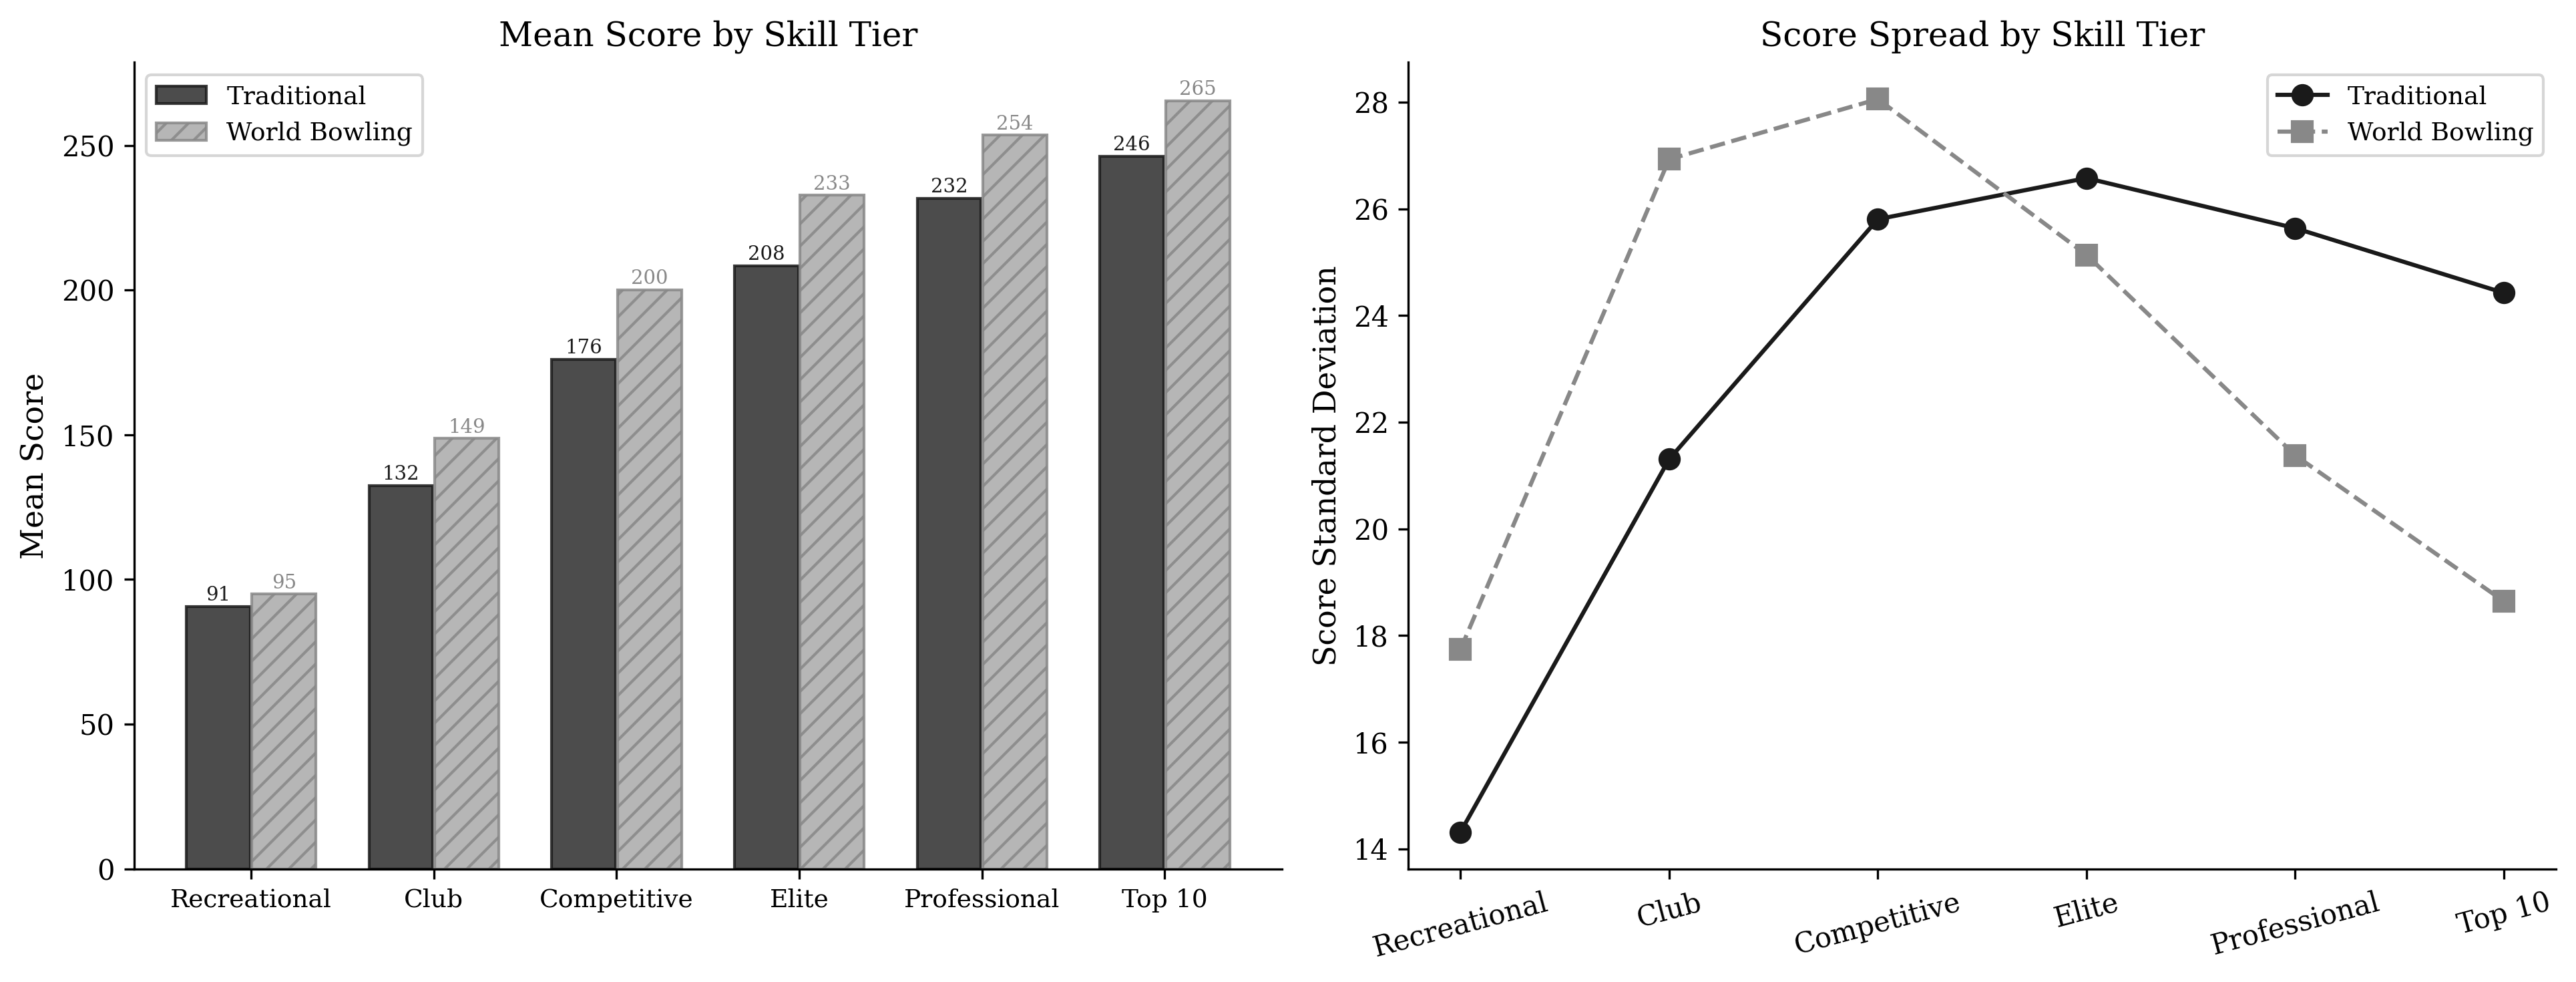
\includegraphics[width=1\linewidth,height=\textheight,keepaspectratio]{../figures/fig9_mean_scores_tiers.png}

}

\caption{\label{fig-tiermeans}Left: mean scores by skill tier. Right:
score standard deviation (note the crossover between systems).}

\end{figure}%

\section{The Score Spread Crossover}\label{the-score-spread-crossover}

\subsection{Standard Deviation as a Function of
Skill}\label{standard-deviation-as-a-function-of-skill}

A critical observation emerges from the simulation: the standard
deviation of scores under each system behaves differently as a function
of player skill.

Under World Bowling, score standard deviation peaks at low-to-moderate
skill levels (SD \(\approx\) 28 at competitive level) and then
\textbf{decreases monotonically} as skill increases, reaching SD
\(\approx\) 18.6 at the Top 10 level. This compression occurs because
high-skill World Bowling games converge toward the maximum of 300. With
most frames scoring 30 (strike), the remaining variance comes only from
occasional non-strikes.

Under traditional scoring, standard deviation increases with skill
through the competitive range and remains elevated (SD \(\approx\) 25.7
at professional, \(\approx\) 24.4 at Top 10). This is because the
compounding bonus structure amplifies the consequences of each
non-strike: a single open frame in an otherwise perfect game costs
substantially more under traditional scoring than under World Bowling,
maintaining score spread even at elite levels.

\subsection{The Crossover Point}\label{the-crossover-point}

We sweep strike rate continuously from 10\% to 80\% and compute score
standard deviation under each system. The two curves cross at a strike
rate of \textbf{48.7\%} (95\% bootstrap confidence interval
48.2\%--49.1\%, from 500 resamples of the simulated games). Below this
threshold, World Bowling produces greater score spread; above it,
traditional scoring produces greater spread.

It is tempting to read this crossover as a crossover in
\emph{discrimination}, with World Bowling separating players better
below 50\% and traditional scoring better above it. That reading is
wrong, and correcting it is the central methodological point of this
section. Standard deviation measures how wide the score distribution is,
not how much of that width reflects genuine differences in player
ability. A scoring system can inflate its standard deviation purely by
amplifying the consequences of a single lucky or unlucky ball, which is
noise, not skill. The next two subsections decompose the spread into
signal and noise and show that, on the axis of raw skill, the extra
spread traditional scoring carries at elite levels is mostly the latter.
The crossover is best understood as a statement about score
\emph{granularity and margins}, the size of the gaps between scores,
rather than about how reliably a single game ranks two players.

\begin{figure}[htbp]

\centering{

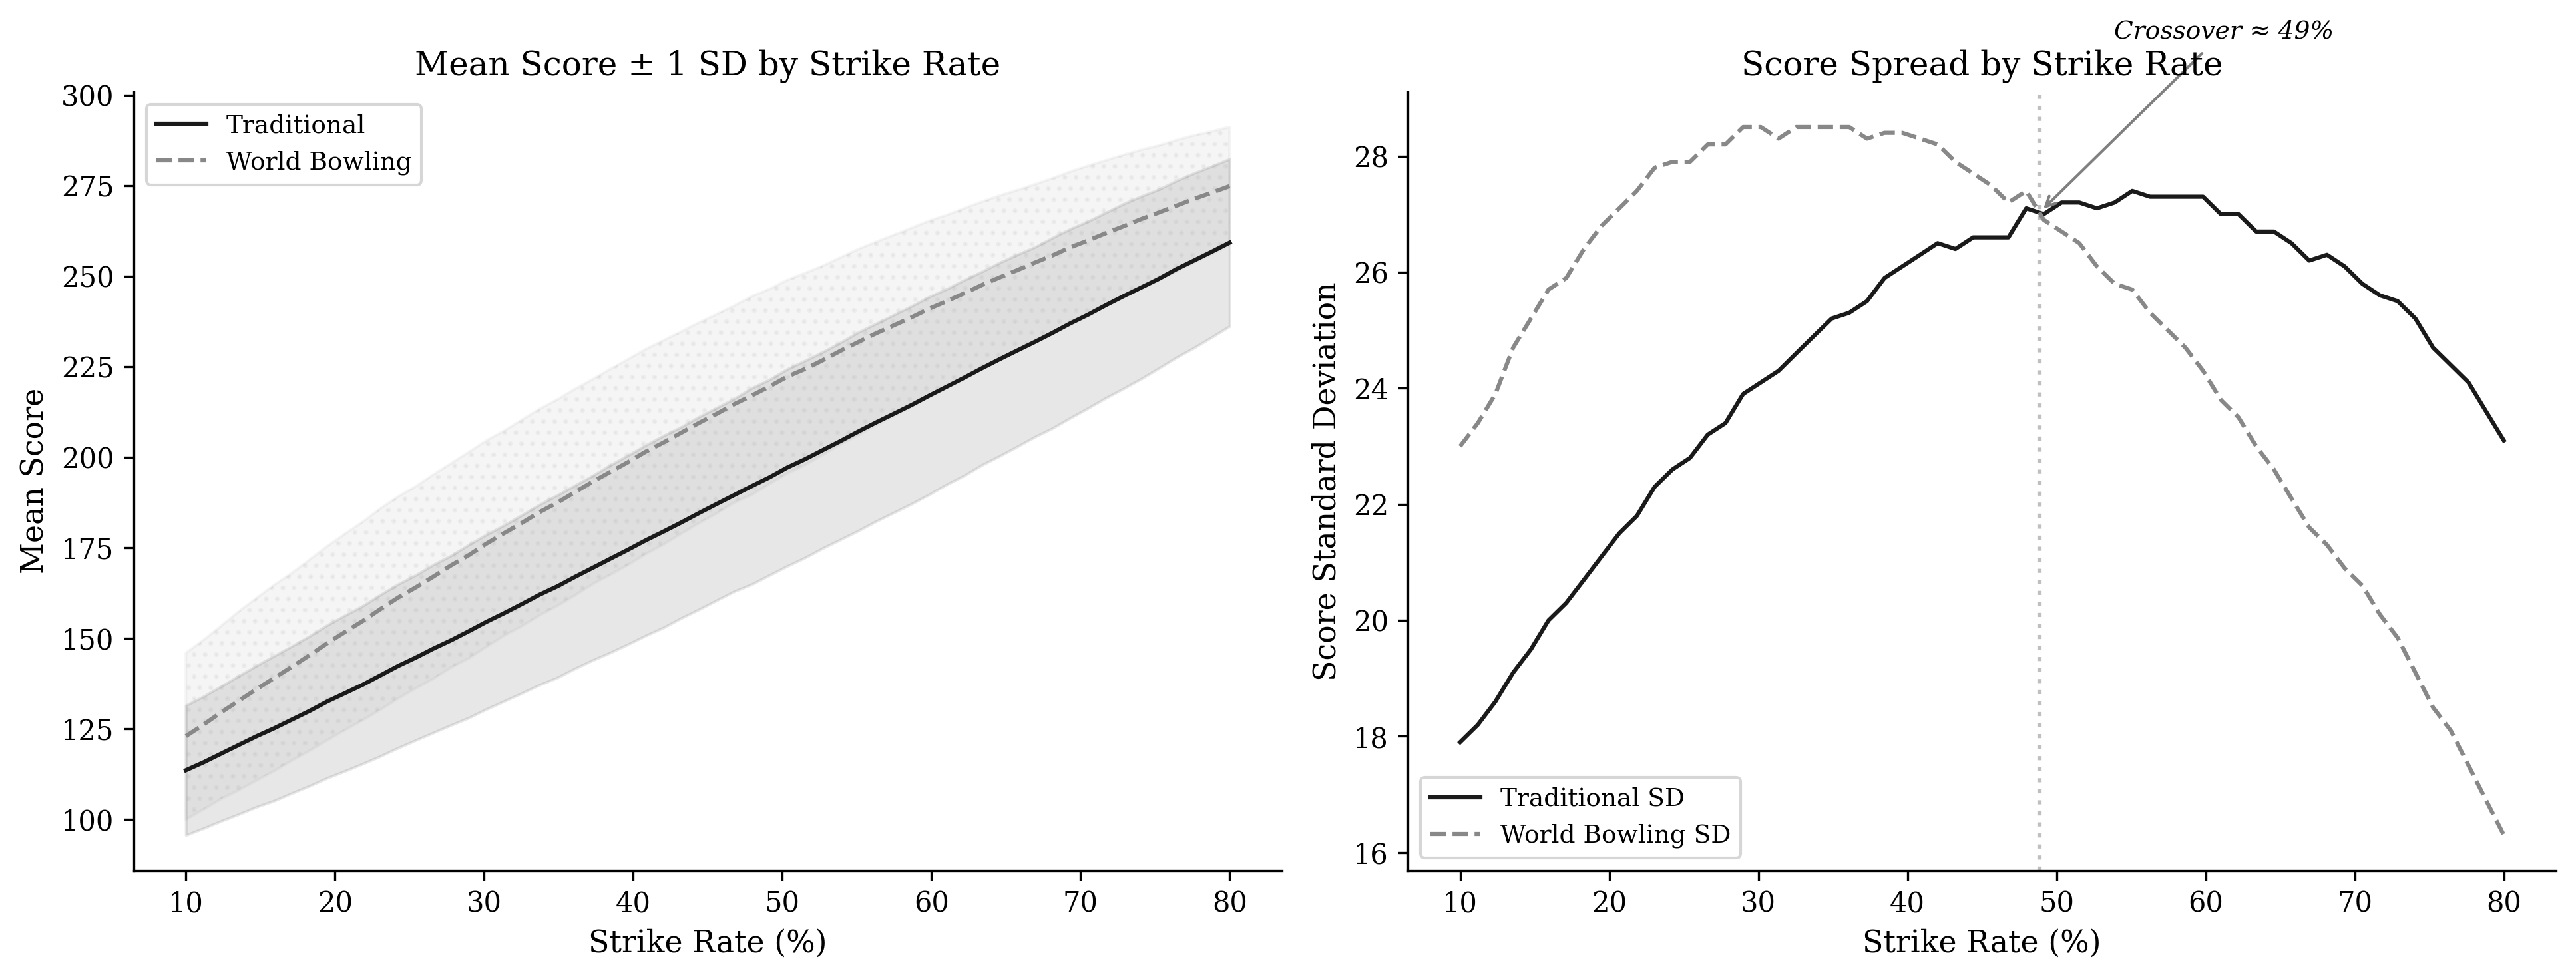
\includegraphics[width=1\linewidth,height=\textheight,keepaspectratio]{../figures/fig10_crossover_analysis.png}

}

\caption{\label{fig-crossover}Left: mean score \(\pm\) 1 SD by strike
rate under both systems. Right: score standard deviation as a function
of strike rate, showing the crossover at approximately 49\% (bootstrap
95\% CI 48.2\%--49.1\%). Note that this is a crossover in score spread,
not in discrimination of skill; see Figure~\ref{fig-reliability}.}

\end{figure}%

\subsection{Signal versus Noise: A Reliability
Analysis}\label{signal-versus-noise-a-reliability-analysis}

The standard deviation of game scores conflates two very different
things: genuine, persistent differences between players (signal) and
game-to-game variation for a single fixed player (noise). A scoring
system that simply magnifies the score impact of a single ball will show
a large standard deviation without discriminating skill any better. To
separate the two, we treat each scoring system as a measurement
instrument and estimate its single-game reliability.

For a target skill level, we construct a population of players whose
true strike rates differ by a realistic amount (a standard deviation of
three strike-rate points, reflecting the within-neighbourhood ability
spread among players nominally at the same level; cf.~the roughly
53\%--66\% posterior strike-rate range across 53 PBA bowlers in
VanDerwerken \& Kenter (\citeproc{ref-vanderwerken2018}{2018})). We
simulate many games per player, score every game under both systems from
the \emph{same} ball sequences, and decompose the total score variance
into a between-player component \(\sigma_B^2\) and a within-player
component \(\sigma_W^2\). The single-game reliability is the intraclass
correlation \(\text{ICC} = \sigma_B^2 / (\sigma_B^2 + \sigma_W^2)\), the
single-measurement ICC under a one-way random-effects model: the
fraction of one game's score variance attributable to real skill
differences. A higher ICC means a single game more reliably identifies
the better player. The absolute level of the ICC depends on the
heterogeneity of the reference population (here a three-point standard
deviation in true strike rate), so it is the comparison between systems,
not the level, that is the result of interest; the small remaining
point-to-point variation in Figure~\ref{fig-reliability} is Monte Carlo
error.

Two findings emerge (Figure~\ref{fig-reliability}). First, the two
systems have nearly identical single-game reliability at every skill
level: the ICC estimates differ by less than 0.01 at strike rates above
roughly 15\%, and by at most 0.025 at the lowest recreational levels,
where World Bowling is if anything marginally the more reliable measure.
On the axis of raw skill, traditional scoring is no better at separating
players than World Bowling. Second, the variance decomposition explains
why traditional scoring's larger elite-level spread does not buy
discrimination: at the top of the range, almost all of the extra spread
is noise. At a 78\% strike rate, traditional scoring's within-player
(noise) standard deviation is about 24 points against World Bowling's
17, while the between-player (signal) standard deviations are comparable
and small (roughly 6 versus 4 points). The amplifying bonus structure
inflates noise and signal together, leaving their ratio, and hence
reliability, essentially unchanged.

This result aligns with the between-tier comparison: across adjacent
skill tiers, both systems produce nearly identical Cohen's \(d\) effect
sizes, from 2.3 (recreational vs club) down to 0.6 (professional vs Top
10), matching to within 0.03 at every boundary. Whether one measures
discrimination between tiers or reliability within a population, the two
systems are equivalent on raw skill. The case for traditional scoring
cannot rest on the standard-deviation crossover, and we do not rest it
there.

\begin{figure}[htbp]

\centering{

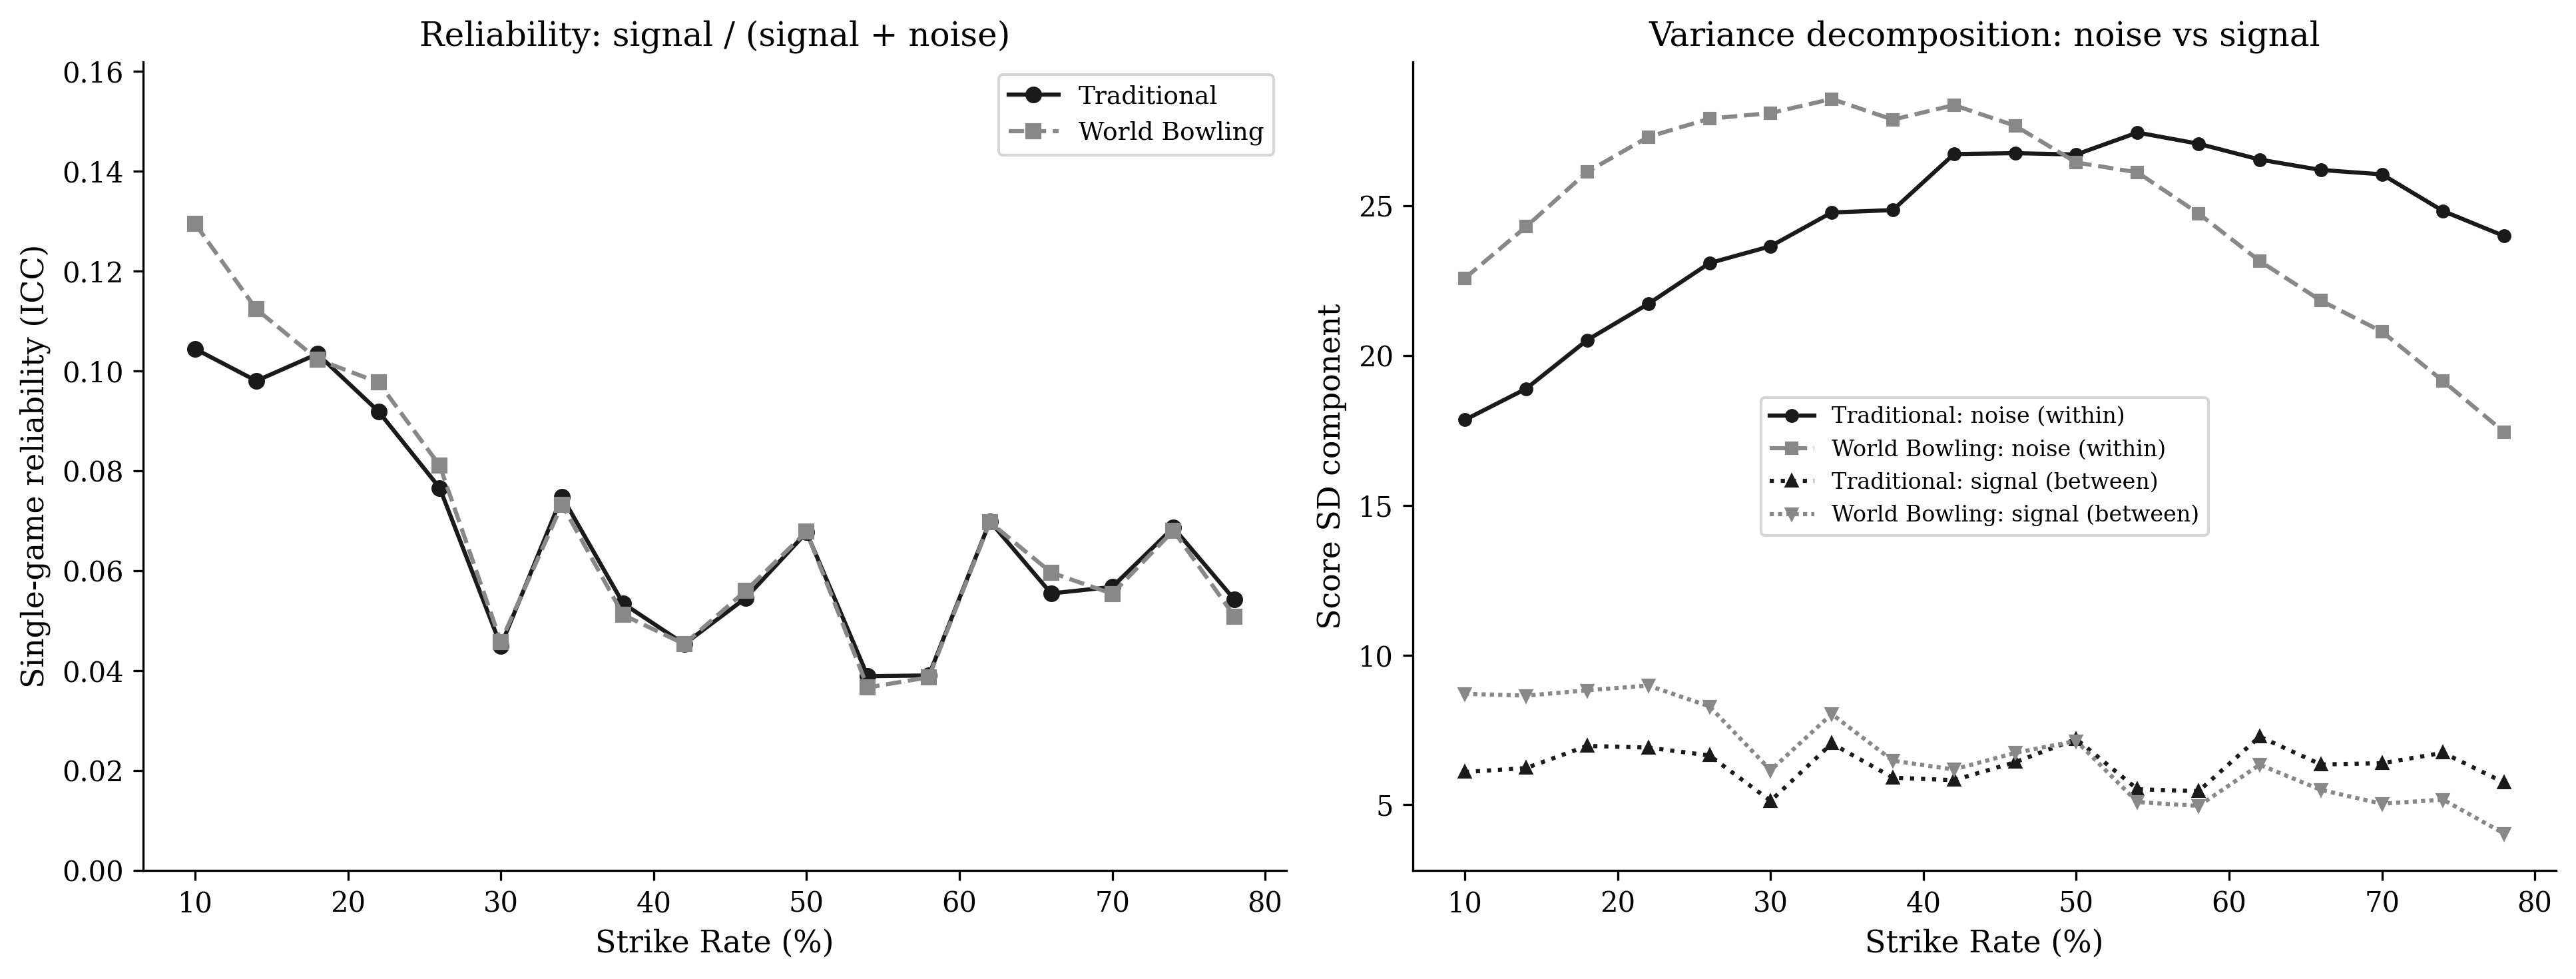
\includegraphics[width=1\linewidth,height=\textheight,keepaspectratio]{../figures/fig14_reliability.png}

}

\caption{\label{fig-reliability}Left: single-game reliability (ICC) as a
function of strike rate. The two systems track each other across the
entire skill range. Right: the variance decomposition. At elite levels
the within-player noise component diverges (traditional scoring is
noisier) while the between-player signal component stays comparable, so
traditional scoring's larger spread is mostly amplified noise.}

\end{figure}%

\subsection{Discriminating Streakiness at Fixed
Skill}\label{discriminating-streakiness-at-fixed-skill}

If the two systems are equally reliable on raw skill, where does
commutativity actually cost something? Precisely where Proposition 1
predicts: in measuring \emph{how} a player arranges a fixed number of
strikes. To isolate this, we hold the marginal strike rate constant and
vary only the lag-1 autocorrelation \(\phi\) of the strike indicator,
the tendency to throw strikes in runs rather than scattering them. A
two-state Markov chain lets us set any autocorrelation while keeping the
expected strike count fixed, so two players with different \(\phi\) are
identical in raw skill and differ only in streakiness. The magnitude
range we sweep (\(\phi\) up to 0.35) spans the hot-hand effect sizes
reported for professional bowlers by VanDerwerken \& Kenter
(\citeproc{ref-vanderwerken2018}{2018}).

The contrast is stark (Figure~\ref{fig-streakiness}). Across a
population of players who share a 66\% strike rate but differ in
streakiness, a player's mean traditional score correlates with true
streakiness at \(r = 0.49\), while the World Bowling correlation is
\(r = -0.04\), indistinguishable from zero. Comparing the extremes
directly, a maximally streaky player (\(\phi = 0.35\)) outscores a
streak-free player (\(\phi = 0\)) of identical raw skill by about seven
points under traditional scoring (235.5 vs 228.6; Cohen's \(d = 0.23\)),
but by nothing under World Bowling (250.6 vs 251.2; \(d = -0.02\)).
World Bowling is not merely noisier at detecting streakiness; it is
structurally incapable of detecting it, exactly as commutativity
requires. This, and not the spread crossover, is the discrimination that
current-frame scoring discards.

\begin{figure}[htbp]

\centering{

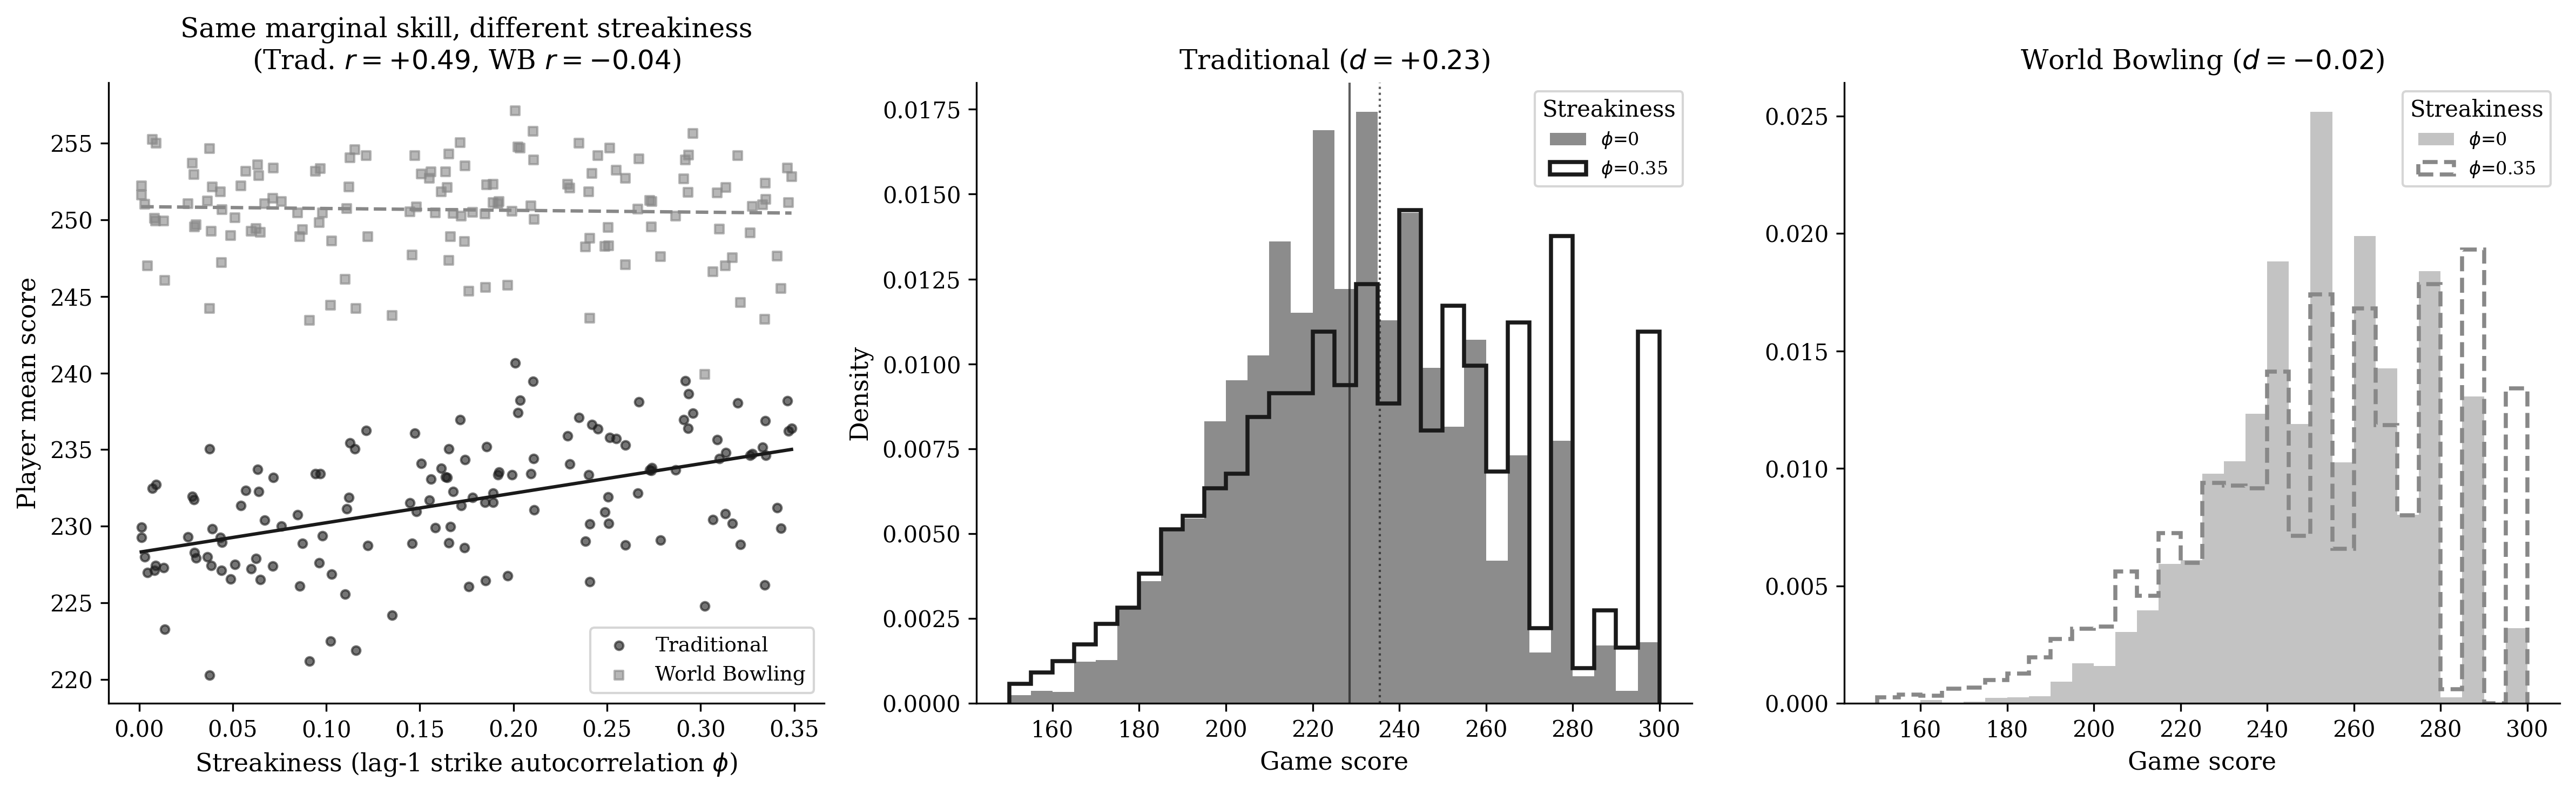
\includegraphics[width=1\linewidth,height=\textheight,keepaspectratio]{../figures/fig15_streakiness.png}

}

\caption{\label{fig-streakiness}Left: player mean score against true
streakiness (\(\phi\)) for a population of players who share an
identical 66\% strike rate. Traditional scores rise with streakiness;
World Bowling scores are flat. Middle and right: game-score
distributions for a streak-free and a maximally streaky player of
identical raw skill, under traditional scoring and World Bowling
respectively. Traditional scoring shifts; World Bowling does not.}

\end{figure}%

The effect is specific to strikes. Repeating the experiment on the spare
dimension, holding the strike process independent and instead clustering
spare \emph{conversions} at a fixed marginal conversion rate, produces
no signal under either system (traditional \(r = 0.02\), World Bowling
\(r = 0.01\)). Part of this null is mechanical: at elite conversion
rates of 86--92\% there is little variance left to cluster. But the
structural reason is decisive regardless: a strike's bonus looks two
balls ahead and can chain into a following strike, so consecutive
strikes compound, whereas a spare's bonus looks only one ball ahead and
never chains into another bonus. Spare conversion is a genuine skill,
and both systems measure it about equally; but only the
\emph{arrangement} of strikes, not of spares, carries sequencing
information, and only traditional scoring records it.

\subsection{Compounding over a Series}\label{compounding-over-a-series}

The per-game streakiness effect is real but moderate (\(d = 0.23\)).
Competition, however, is decided over multi-game blocks and tournaments,
and an independent per-game advantage compounds: the expected
total-score gap grows linearly in the number of games while its standard
deviation grows only as the square root, so the series-level effect size
grows as \(\sqrt{n}\). Figure~\ref{fig-series} traces this for our two
identical-skill players, one streak-free and one streaky. Under
traditional scoring the streaky player's probability of winning a
head-to-head series rises from 57\% over a single game to 67\% over a
six-game block and 90\% over a 48-game tournament, and the series effect
size grows from \(d = 0.26\) to \(d = 1.79\). Under World Bowling the
same player's win probability never leaves the neighbourhood of chance
(53\% even at 48 games). These figures should be read as upper bounds on
the practical stakes: they contrast the extremes of the swept
streakiness range (\(\phi = 0.35\) versus \(\phi = 0\)), and the
between-player dispersion of streakiness in real professional
populations is not yet established. If the population spread of \(\phi\)
is narrower than the range swept here, the win probabilities move toward
chance proportionally. Subject to that caveat, a property that looks
minor in a single game becomes, over the span of a real competition,
frequently decisive under traditional scoring and nearly invisible under
World Bowling.

\begin{figure}[htbp]

\centering{

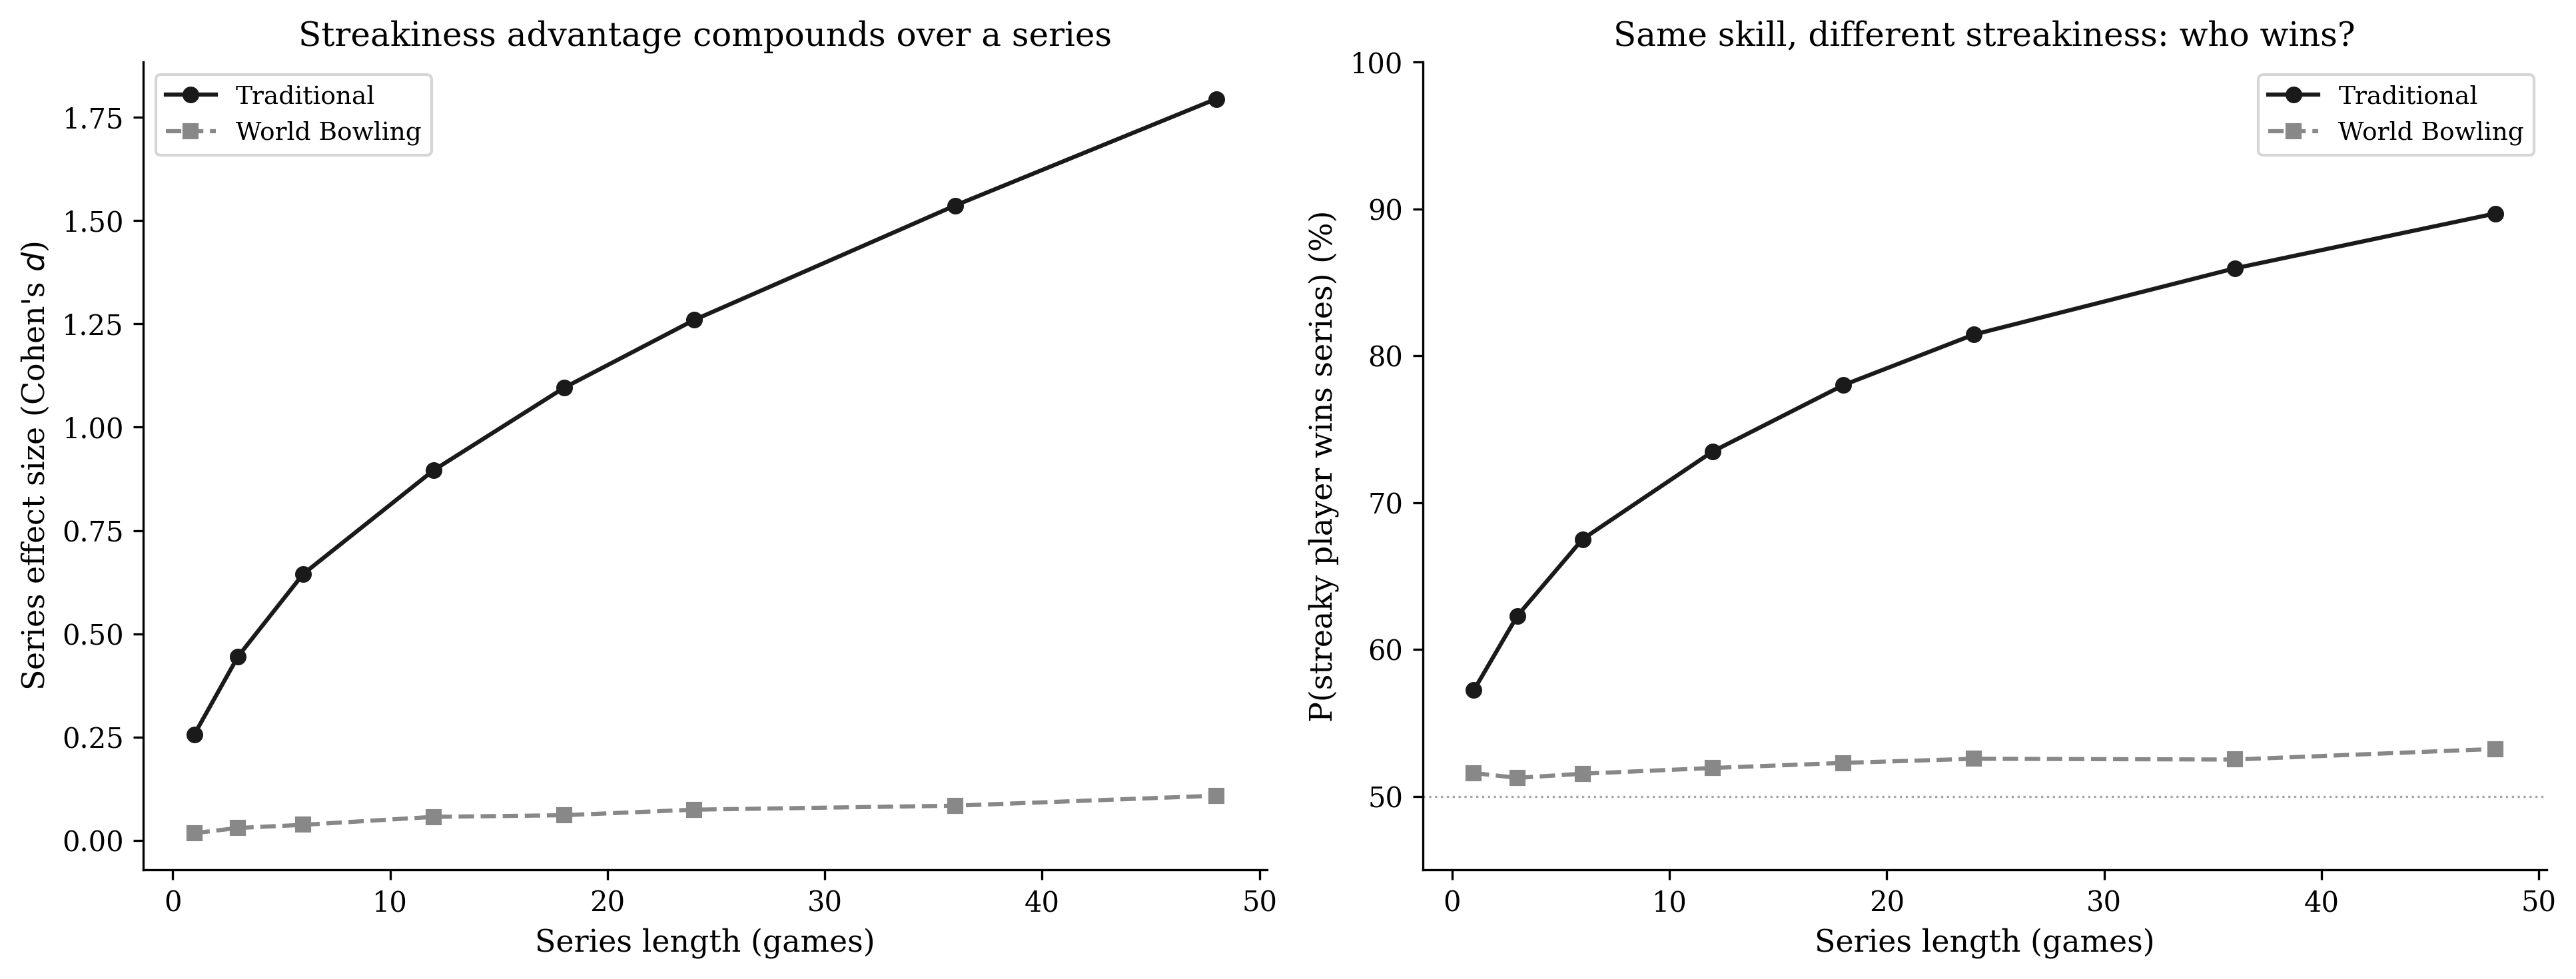
\includegraphics[width=1\linewidth,height=\textheight,keepaspectratio]{../figures/fig16_series_compounding.png}

}

\caption{\label{fig-series}Left: the series-level effect size (Cohen's
\(d\)) separating a streaky player from a streak-free player of
identical 66\% strike rate, as a function of series length; it grows as
\(\sqrt{n}\) under traditional scoring and stays near zero under World
Bowling. Right: the probability that the streaky player wins a
head-to-head series of the given length.}

\end{figure}%

\section{Professional-Level Sequence
Analysis}\label{professional-level-sequence-analysis}

\subsection{Specific Sequence
Comparisons}\label{specific-sequence-comparisons}

To illustrate the practical consequences at the professional level, we
compute scores for sequences representative of elite play:

\begin{longtable}[]{@{}llll@{}}
\caption{Professional-level sequence comparisons. The systems agree at
the extremes but diverge substantially for mixed
sequences.}\label{tbl-proseq}\tabularnewline
\toprule\noalign{}
Sequence & Traditional & World Bowling & Difference \\
\midrule\noalign{}
\endfirsthead
\toprule\noalign{}
Sequence & Traditional & World Bowling & Difference \\
\midrule\noalign{}
\endhead
\bottomrule\noalign{}
\endlastfoot
Perfect game (12 strikes) & 300 & 300 & 0 \\
10 strikes + spare(7,3) + 7 & 287 & 300 & −13 \\
8 strikes + 2 spares(7,3) + 7 & 261 & 274 & −13 \\
6 spares then 4 strikes + X,X & 215 & 210 & +5 \\
4 strikes then 6 spares + 5 & 195 & 210 & −15 \\
Alternating strike/spare × 5 & 200 & 225 & −25 \\
All spares (5,5) + 5 & 150 & 150 & 0 \\
\end{longtable}

Two patterns are notable. First, the systems agree at the extremes
(perfect game and all spares) but diverge substantially for the mixed
sequences that constitute the vast majority of professional games.
Second, the \emph{direction} of the difference depends on the sequence:
traditional scoring rewards sequences with consecutive strikes more than
World Bowling does, while World Bowling rewards isolated strikes more.
The traditional system encodes \emph{how} the strikes were arranged;
World Bowling treats them as interchangeable.

\begin{figure}[htbp]

\centering{

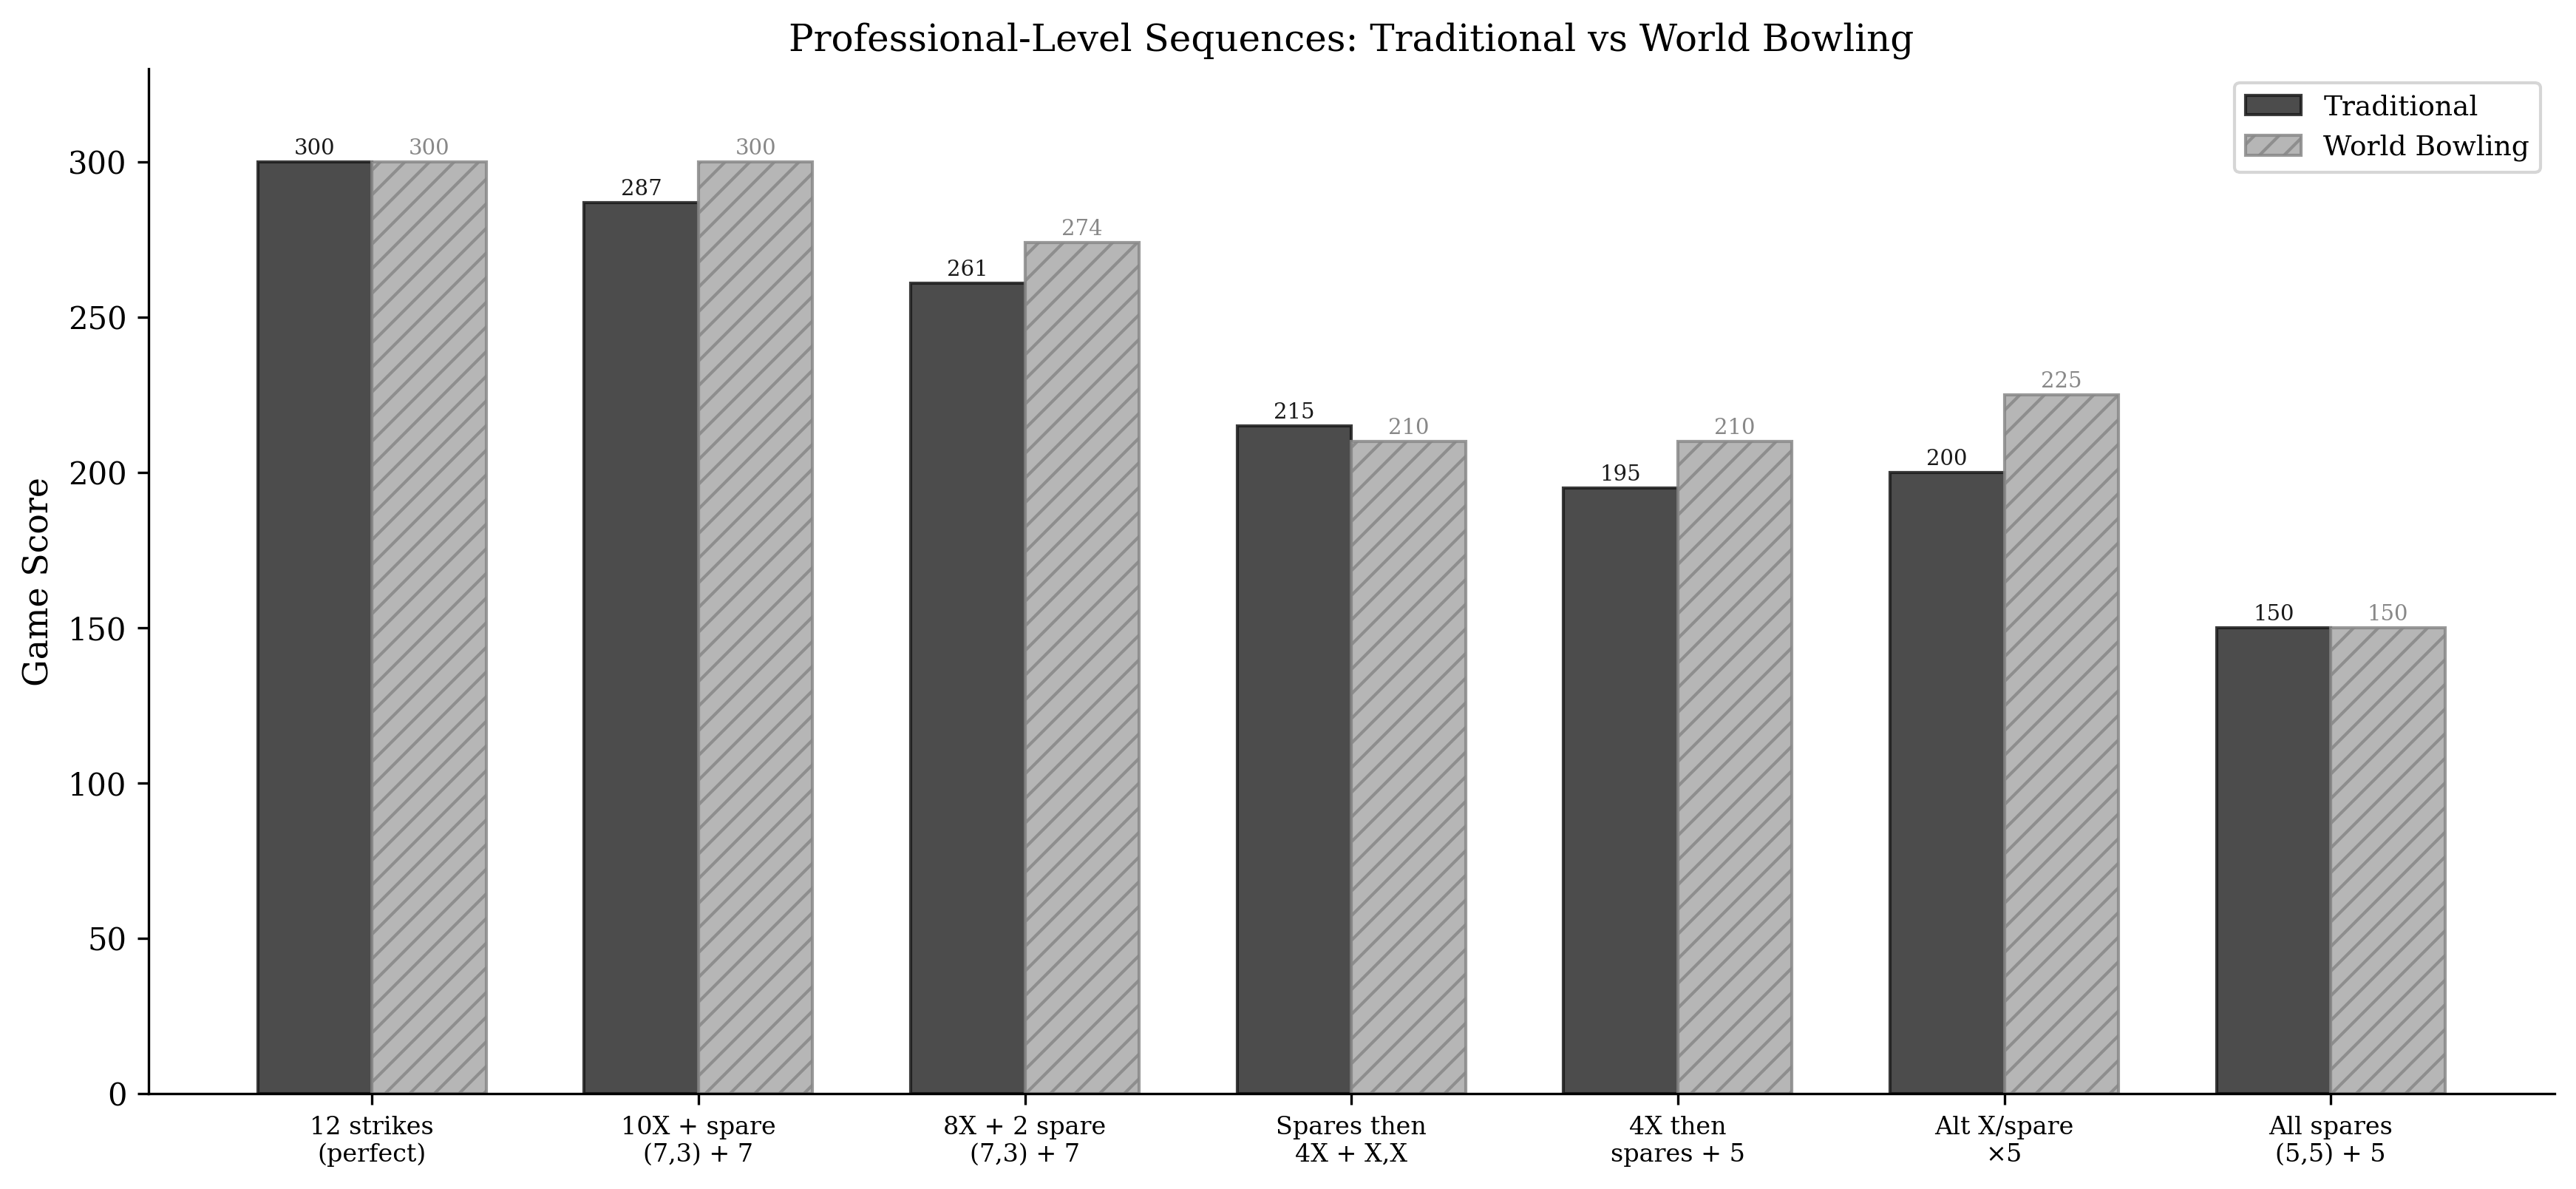
\includegraphics[width=1\linewidth,height=\textheight,keepaspectratio]{../figures/fig11_professional_sequences.png}

}

\caption{\label{fig-proseq}Professional-level sequence comparison under
both scoring systems.}

\end{figure}%

\subsection{The Fourth-to-Fifth Strike
Problem}\label{the-fourth-to-fifth-strike-problem}

Consider a professional bowler who has thrown four consecutive strikes.
Under traditional scoring, the fifth strike is worth substantially more
than under World Bowling (+21 from the compounding bonus structure),
because it both earns its own bonus and retroactively increases the
value of the preceding strikes. Under World Bowling, the fifth strike is
worth exactly the same as if it were the first strike of the game (30
points, net +21 over an average open frame).

This flattening of the reward gradient at the professional level is not
a simplification; it is a loss of information. The ability to extend a
strike run from four to five frames is one of the most difficult and
competitively meaningful feats in professional bowling. Traditional
scoring encodes that difficulty in the score. World Bowling does not.

\section{Discussion}\label{discussion}

\subsection{What Scoring Systems
Measure}\label{what-scoring-systems-measure}

A scoring system is a function from a sequence of physical performances
to a number. The properties of that function determine what the number
communicates about the athlete's skill. This perspective connects to the
broader theory of proper scoring rules, where the design of a
measurement function determines whether it faithfully elicits the
quantity it claims to measure (\citeproc{ref-gneiting2007}{Gneiting \&
Raftery, 2007}). Two scoring systems can agree on the maximum possible
score (both systems peak at 300 for a perfect game) while disagreeing
significantly on how they encode the path to that maximum.

Traditional bowling scoring encodes two distinct performance qualities
simultaneously: the absolute pin count (how many pins were knocked down)
and the sequencing of that performance (whether those knockdowns were
concentrated in consecutive frames or distributed across the game).
World Bowling scoring encodes only the first.

\subsection{The Commutativity
Trade-off}\label{the-commutativity-trade-off}

The commutativity of World Bowling scoring (Proposition 1) is its
defining feature. It makes the system simple to compute and explain. But
commutativity in a scoring function means that sustained performance is
not valued above distributed performance. In most competitive sports,
consecutive success is considered more difficult than the same success
spread over time. A tennis player who wins six consecutive games
demonstrates something different from one who wins six non-consecutive
games. Traditional bowling scoring agrees with this intuition. World
Bowling scoring does not.

\subsection{Is Streakiness a Skill, and Should It Be
Rewarded?}\label{is-streakiness-a-skill-and-should-it-be-rewarded}

Our central empirical claim is that traditional scoring rewards
streakiness and World Bowling does not. Whether that is a virtue depends
on a question our data cannot fully settle: is the tendency to throw
consecutive strikes a stable, skill-based attribute, or an artefact of
luck and changing conditions? The hot-hand question, whether streaks
reflect a causal change in player state or merely the perception of one
(\citeproc{ref-gilovich1985}{Gilovich et al., 1985}), is pointed on
exactly this in bowling. Dorsey-Palmateer \& Smith
(\citeproc{ref-dorseypalmateer2004}{2004}) find positive autocorrelation
in strike sequences, but Yaari \& Eisenmann
(\citeproc{ref-yaari2012}{2012}), analysing a large body of data,
conclude that the correlation reflects association with recent results
rather than a causal ``hot hand,'' and is plausibly driven by varying
lane conditions, equipment, and form across a session rather than by
momentum within a player. We take this seriously, because it bears
directly on whether rewarding streaks rewards skill or amplifies noise.

We make three points in response. First, our finding is robust to the
interpretation: regardless of \emph{why} strikes cluster, traditional
scoring records the clustering and World Bowling discards it. The
structural fact stands. Second, even on the conditions-based reading,
the within-game arrangement of strikes is not purely random with respect
to the player. A bowler who reads a lane, adjusts, and converts a
favourable stretch into a run of strikes is exercising a competitive
capability, even if ``momentum'' is the wrong mechanism for it; the
relevant question for a scoring system is whether the achievement
happened, not which latent process produced it. Third, and most
importantly, whether sequencing \emph{ought} to count is a normative
choice about what the sport wishes to measure, not a fact to be
discovered. Our contribution is to make that choice explicit and
quantified: traditional scoring treats sequencing as part of
performance, World Bowling treats it as irrelevant, and a governing body
should choose between them knowing precisely which property it is
keeping or discarding. We note the streakiness signal we measure
(\(r = 0.49\) at the population level, \(d = 0.23\) between extremes) is
real but moderate, so the practical stakes of this choice, while
genuine, should not be overstated.

\subsection{The Appropriate Domain for Each
System}\label{the-appropriate-domain-for-each-system}

We do not argue that current-frame scoring lacks merit. For recreational
participants, its simplicity and accessibility represent genuine
improvements over traditional scoring. The simulation results support
this: below approximately 50\% strike rate, World Bowling produces
\emph{greater} score spread, and its simpler computation removes a
barrier to casual participation. The higher Shannon entropy of the World
Bowling distribution (5.94 vs 5.81 bits; Shannon
(\citeproc{ref-shannon1948}{1948})) reflects this wider spread, since
entropy here measures dispersion rather than discrimination, a
distinction our reliability analysis makes concrete. A casual player's
score therefore more directly reflects their raw pin count without the
amplifying effect of bonus compounding.

Our argument is narrower, and the reliability analysis sharpens it. At
the competitive and professional levels, where strike rates exceed 50\%
and the ability to string consecutive strikes is a distinguishing skill,
current-frame scoring is not a worse measure of raw skill, but it is
blind to the sequencing dimension that traditional scoring records
(Figure~\ref{fig-streakiness}). The spread crossover at approximately
49\% strike rate is not the basis of this argument; it marks where the
score scale changes character, not where discrimination of skill
reverses.

Nor is the choice binary. Traditional and current-frame scoring are two
points in a design space, not the whole space. A governing body that
valued both accessibility and sequencing could adopt a hybrid:
current-frame base scoring with an explicit consecutive-strike bonus
(for example, a fixed supplement for a double or turkey) would recover
much of the sequencing signal at a fraction of traditional scoring's
computational complexity. Our framework supplies the tools to evaluate
such designs: enumerate the distribution, measure the sequence
sensitivity, and estimate the reliability before changing the rules.
Mapping that design space is a natural extension of this work.

\subsection{Score Compression at the Elite
Level}\label{score-compression-at-the-elite-level}

The high-score compression shown in Table~\ref{tbl-compression},
combined with the decreasing standard deviation under World Bowling at
high skill levels (Figure~\ref{fig-crossover}), narrows the score range
available to separate elite players. At the Top 10 professional level,
World Bowling's score SD of 18.6 compared to traditional's 24.4 means
roughly 24\% less score spread, with a similar gap at the professional
tier (SD 21.4 vs 25.7). It is important to state precisely what this
does and does not imply. As the reliability analysis showed
(Figure~\ref{fig-reliability}), the wider traditional spread is mostly
amplified noise, so the two systems rank players about equally well in
any single game; the compression does not, by itself, make World Bowling
a worse discriminator of raw skill. What compression does affect is the
granularity of the score scale: with scores packed into a narrower band
and 290--299 unreachable, more distinct performances collapse onto the
same number, leaving fewer score values to register fine differences and
break ties over a tournament. The substantive loss is not resolution of
raw skill but resolution of \emph{sequencing}, which
Figure~\ref{fig-streakiness} shows traditional scoring records and World
Bowling cannot.

\subsection{End-Loading and the Perception of
Unfairness}\label{end-loading-and-the-perception-of-unfairness}

Sequence sensitivity has a second, less obvious asymmetry beyond the
reward gradient: under traditional scoring, a ball thrown late in the
game contributes more to the total than the same ball thrown early.
Every ball enters the score up to three times, once in its own frame and
once in each of up to two preceding frames as a bonus, so the balls of
frame 1 enter exactly one frame-score while the balls of frame 9 can
enter three. A weak frame is correspondingly cheaper early than late.
Holding the frame composition fixed, a player who throws nine strikes
and one spare (5,5) scores 290 if the spare comes first but 270 if it
comes last; with nine strikes and one open frame (9,0), the scores are
279 and 267. Under World Bowling both orderings score identically (285
and 279 respectively). The tenth-frame open is, structurally, the most
expensive mistake in traditional scoring.

This end-loading is the source of a recurring informal complaint about
traditional scoring: two players who throw identical frames in different
orders receive different scores, and the difference is not symmetric,
because the system forgives a slow start more readily than a weak
finish. What the complaint identifies is not a flaw but a design
property. Traditional scoring places a premium on the closing frames,
much as other sports reward performance in high-leverage moments.
Whether this clutch premium is desirable, whether the sport wants the
tenth frame to matter most, is a normative question, and it is the same
question the sequencing result poses from another angle: current-frame
scoring is neutral to order, treating a strike in frame 1 and a strike
in frame 10 as identical events.

The hot-hand literature, extensively reviewed by Bar-Eli et al.
(\citeproc{ref-bareli2006}{2006}) and investigated in bowling
specifically by Yaari \& Eisenmann (\citeproc{ref-yaari2012}{2012}) and
Dorsey-Palmateer \& Smith (\citeproc{ref-dorseypalmateer2004}{2004}),
documents that strike sequences are autocorrelated rather than
independent, though it disputes whether the cause is a causal hot hand
or shared dependence on session conditions. Either way, both the
sequencing and the end-loading exist in the scoring record; whether a
scoring system should reflect them is the normative question discussed
above.

\subsection{The 290--299 Gap as a Design
Artefact}\label{the-290299-gap-as-a-design-artefact}

The impossibility of World Bowling scores in the range 290--299 is
mathematically unavoidable given the system's design. It is a direct
consequence of the discrete jump between the maximum achievable score
with 9 strikes (289) and the minimum score with 10 strikes (300). This
gap means that a bowler who throws nine strikes and one near-perfect
spare cannot be scored above 289, while one who converts that spare to a
tenth strike jumps directly to 300. The scoring cliff at the top of the
range is not a feature of athletic performance; it is an artefact of
linear frame independence.

\subsection{Robustness Across Simulation
Models}\label{robustness-across-simulation-models}

Our base simulation assumes frame-to-frame independence: each ball's
outcome depends only on the player's fixed skill parameters, not on
preceding results. This is deliberately conservative. The hot hand
literature in bowling
(\citeproc{ref-dorseypalmateer2004}{Dorsey-Palmateer \& Smith, 2004};
\citeproc{ref-yaari2012}{Yaari \& Eisenmann, 2012}) provides empirical
evidence that consecutive strikes are positively correlated (a
``momentum'' or streakiness effect) which an independence model ignores.

To test the sensitivity of our conclusions to this assumption, we
compare three simulation models of increasing realism: the independent
base case, a simple momentum model (±5\% strike probability shift after
strikes/opens), and a first-order Markov chain with leave-dependent
spare difficulty (Section 6.2). Figure~\ref{fig-robustness} shows the
score standard deviations and the SD gap (traditional minus World
Bowling) across all six skill tiers under each model. Two observations
are immediate. First, all three models agree on the \emph{direction} of
the effect at every tier: World Bowling provides more spread below
competitive level, and traditional scoring provides more spread above
it. The crossover point is robust to model choice. Second, the more
realistic models produce \emph{larger} gaps at the professional and Top
10 levels: the Markov model yields a traditional scoring advantage of
+5.8 SD points at the Top 10 tier, compared to +4.1 under independence.
The independence assumption is therefore conservative: any realistic
model of sequential dependence amplifies the effect.

\begin{figure}[htbp]

\centering{

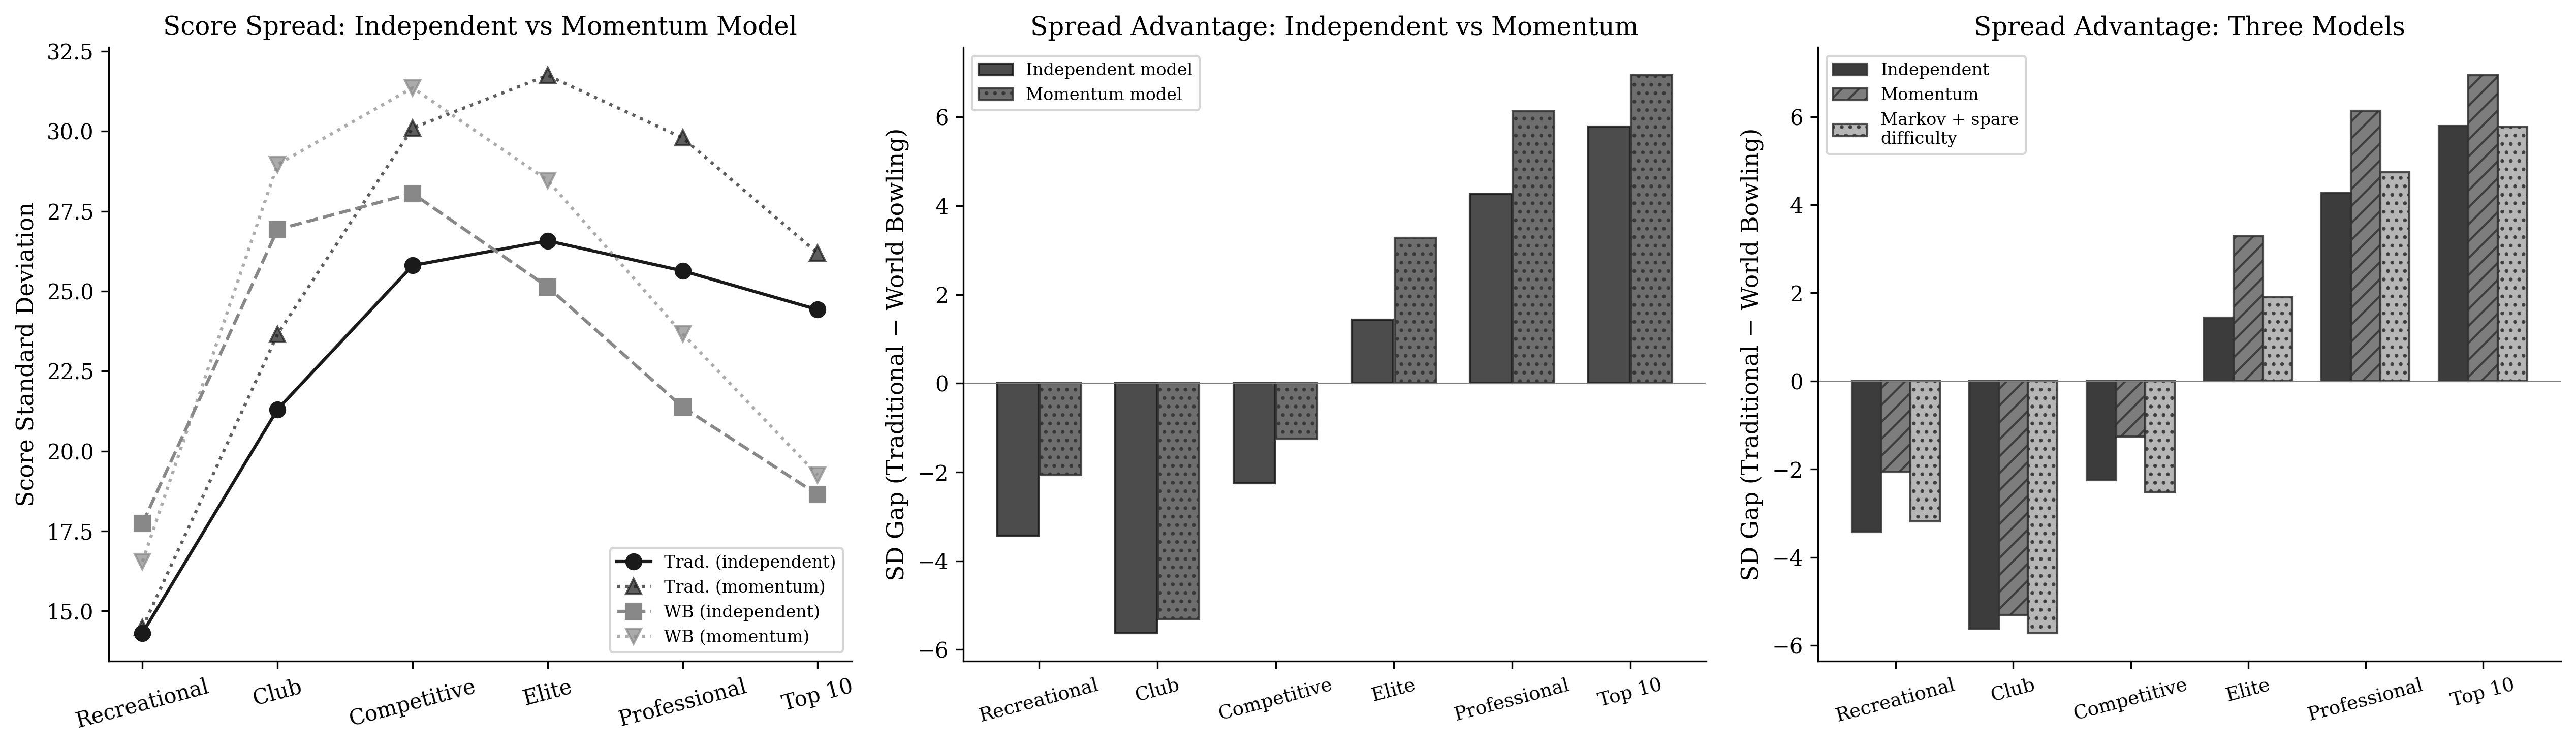
\includegraphics[width=1\linewidth,height=\textheight,keepaspectratio]{../figures/fig12_model_robustness.png}

}

\caption{\label{fig-robustness}Robustness across simulation models.
Left: score standard deviation by skill tier under independent and
momentum models. Middle: SD gap (traditional minus World Bowling) by
tier under each. Right: SD gap under all three models, including the
Markov chain with spare difficulty. More realistic models amplify the
traditional scoring advantage at elite tiers.}

\end{figure}%

\subsection{Limitations and Future
Work}\label{limitations-and-future-work}

This paper has several limitations that suggest directions for future
work. First, the simulation uses a parametric skill model rather than
real game data. As a face-validity check, a population mixture of
bowlers with a mean strike rate of 54\% and an ability standard
deviation of eight strike-rate points reproduces the pooled PBA moments
reported by McCarthy (\citeproc{ref-mccarthy2011}{2011}) closely:
simulated mean 204.4 and standard deviation 31.5, against the published
205.65 and 31.91. This confirms that the model reproduces the real
aggregate score distribution and not merely its mean, but it is not a
substitute for ball-by-ball validation. We want to be precise about the
scope of this limitation: the calibration validates the model's
\emph{marginal} behaviour (score means and spreads by tier), while the
paper's headline claims concern \emph{sequential} structure, and the
sequential inputs, the Markov transition ratios and the spare
leave-class probabilities, are assumed from published ranges rather than
fitted to ball-by-ball data. Applying both scoring systems to a database
of actual PBA tournament games, and re-estimating the reliability and
streakiness results on real strike sequences, would provide a far
stronger empirical anchor, and it is the most important extension of
this work. Second, while the Markov chain model captures first-order
sequential dependence, more sophisticated models incorporating fatigue,
lane oil breakdown, and frame-specific strategy could further refine the
magnitude estimates. Third, we show that the per-game sequencing effect
compounds over a multi-game series under an independence assumption
(Figure~\ref{fig-series}), but a fuller tournament-format treatment,
incorporating within-session correlation between games (shared lane
conditions and form), bracket structures, and qualifying cuts, would
sharpen the estimate of how often sequencing actually decides real
competitions. The direction of this effect is genuinely uncertain: if
streakiness is a persistent player attribute, within-session correlation
lets the streaky player's advantage persist across games, making our
estimate conservative; but if streaks are driven by lane conditions
shared with the opponent on the same pair, the \emph{differential}
between players could instead shrink. Fourth, a formal Win Probability
Added (WPA) analysis, computing how each scoring system affects the
probability of winning a head-to-head match at each game state, would
complement the present score-distribution analysis with a
competition-dynamics perspective. The source code accompanying this
paper is designed to support these extensions.

\section{Conclusion}\label{conclusion}

We have demonstrated, through exact combinatorial analysis and
skill-weighted simulation, that traditional and World Bowling scoring
systems differ in mathematically precise and practically significant
ways:

\begin{enumerate}
\def\labelenumi{\arabic{enumi}.}
\item
  \textbf{Traditional scoring is sequence-sensitive.} The order of
  frames matters, and it matters in a way that rewards consecutive
  success. World Bowling scoring is commutative; order is irrelevant.
  Exhaustive permutation analysis shows that the same frame composition
  can produce a score range of up to 39 points under traditional
  scoring, while World Bowling collapses all orderings to a single
  score.
\item
  \textbf{Traditional scoring has a compounding reward gradient for
  consecutive strikes.} Each strike in a string is worth more than an
  isolated strike, creating a non-linear incentive for sustained
  excellence. World Bowling scoring is linear: every strike is worth the
  same regardless of context.
\item
  \textbf{On raw skill the two systems are equally reliable; their
  score-spread curves cross at a 49\% strike rate, but their
  discrimination does not.} A variance decomposition shows nearly
  identical single-game reliability across the entire skill range, and
  the larger spread traditional scoring carries at elite levels (over
  30\% more at the Top 10 tier) is mostly within-player noise. The
  crossover marks a change in the granularity of the score scale, not a
  reversal in how reliably a single game ranks two players. The case for
  traditional scoring does not rest on score spread, and a common
  version of that case is mistaken.
\item
  \textbf{The genuine and exclusive advantage of traditional scoring is
  sequencing discrimination.} At a fixed strike rate, traditional scores
  rise with a player's tendency to string strikes together (population
  correlation 0.49; Cohen's \(d = 0.23\) between the extremes), while
  World Bowling scores stay flat (correlation −0.04). World Bowling is
  not merely a noisier measure of this dimension; by commutativity
  (Proposition 1) it is structurally blind to it. The per-game effect is
  moderate but compounds: as an upper bound, a maximally streaky player
  versus a streak-free player of identical raw skill wins a head-to-head
  48-game tournament about 90\% of the time under traditional scoring,
  against roughly chance (53\%) under World Bowling, with the true
  figure depending on the dispersion of streakiness in the population,
  which is not yet established. The advantage is specific to strikes;
  clustering spare conversions carries no signal under either system.
  This is the property the choice between the two systems actually turns
  on.
\end{enumerate}

The complexity of traditional scoring is not an accident of history. It
is the mechanism by which the system encodes one quality distinctive of
elite bowling: the ability to string consecutive strikes across frames
and across games. Removing that complexity removes that measurement,
while leaving the measurement of raw skill essentially intact.

For governing bodies, tournament organisers, and league administrators,
the practical implication is a clarified trade-off rather than a
verdict. Current-frame scoring loses little in the measurement of raw
skill and gains real simplicity, which makes it well suited to
recreational and casual play. Its cost falls specifically on sequencing:
it cannot distinguish a player who sustains consecutive strikes from one
who scatters the same strikes through a game. Whether elite competition
should reward that sequencing is a normative decision about what the
sport wishes to measure; this paper's contribution is to show precisely
what is kept and what is discarded, so that the decision can be made
deliberately rather than by appeal to score spread.

\section*{Reproducibility}\label{reproducibility}
\addcontentsline{toc}{section}{Reproducibility}

All results in this paper are fully reproducible. The source code, exact
distribution data, and analysis scripts are publicly available at
\url{https://github.com/michael-borck/skill-sequence-scoring}. An
interactive companion website at
\url{https://michael-borck.github.io/skill-sequence-scoring} allows
readers to explore the sequence sensitivity and reward gradient results
directly.

\section*{Acknowledgements}\label{acknowledgements}
\addcontentsline{toc}{section}{Acknowledgements}

All computations were performed in Python using NumPy, Matplotlib, and
SciPy. The manuscript was prepared with Quarto and rendered via
LuaLaTeX. Score distribution computations were verified against
published tables by Balmoral Software.

AI-assisted tools (Anthropic Claude, GitHub Copilot, Google Gemini) were
used during code development, manuscript drafting, and critical review.
All mathematical results, research design, arguments, and editorial
decisions are the author's own.

\section*{References}\label{references}
\addcontentsline{toc}{section}{References}

\protect\phantomsection\label{refs}
\begin{CSLReferences}{1}{0}
\bibitem[\citeproctext]{ref-balmoral}
Balmoral Software. (2019). \emph{All about bowling scores}.
\url{http://www.balmoralsoftware.com/bowling/bowling.htm}.

\bibitem[\citeproctext]{ref-bareli2006}
Bar-Eli, M., Avugos, S., \& Raab, M. (2006). Twenty years of {``hot
hand''} research: Review and critique. \emph{Psychology of Sport and
Exercise}, \emph{7}(6), 525--553.
\url{https://doi.org/10.1016/j.psychsport.2006.03.001}

\bibitem[\citeproctext]{ref-reuters2025wbl}
Chakraborty, A. (2025). \emph{Exclusive: {Betts}-backed {World Bowling
League} to roll out next year}. Reuters.
\url{https://www.reuters.com/sports/cricket/betts-backed-world-bowling-league-roll-out-next-year-2025-06-13/}

\bibitem[\citeproctext]{ref-cooper1990}
Cooper, C. N., \& Kennedy, R. E. (1990). A generating function for the
distribution of the scores of all possible bowling games.
\emph{Mathematics Magazine}, \emph{63}(4), 239--243.
\url{https://doi.org/10.1080/0025570X.1990.11977527}

\bibitem[\citeproctext]{ref-dorseypalmateer2004}
Dorsey-Palmateer, R., \& Smith, G. (2004). Bowlers' hot hands. \emph{The
American Statistician}, \emph{58}(1), 38--45.
\url{https://doi.org/10.1198/0003130042809}

\bibitem[\citeproctext]{ref-gilovich1985}
Gilovich, T., Vallone, R., \& Tversky, A. (1985). The hot hand in
basketball: On the misperception of random sequences. \emph{Cognitive
Psychology}, \emph{17}(3), 295--314.
\url{https://doi.org/10.1016/0010-0285(85)90010-6}

\bibitem[\citeproctext]{ref-gneiting2007}
Gneiting, T., \& Raftery, A. E. (2007). Strictly proper scoring rules,
prediction, and estimation. \emph{Journal of the American Statistical
Association}, \emph{102}(477), 359--378.
\url{https://doi.org/10.1198/016214506000001437}

\bibitem[\citeproctext]{ref-hohn2009}
Hohn, J. L. (2009). \emph{Generalized probabilistic bowling
distributions} {[}Master's thesis{]}. Western Kentucky University.

\bibitem[\citeproctext]{ref-insidethegames2014}
Inside The Games. (2014). \emph{New scoring system introduced for {World
Bowling Tour} finals to try to help sport's {Olympic} ambitions}.
\url{https://www.insidethegames.biz/articles/new-scoring-system-introduced-for-world-bowling-tour-finals-to-try-to-help-sports-olympic-ambitions}.

\bibitem[\citeproctext]{ref-keogh2011}
Keogh, J., \& O'Neill, S. (2011). \emph{A statistical analysis of 10-pin
bowling scores and an examination of the fairness of alternative
handicapping systems}. National University of Ireland, Maynooth.

\bibitem[\citeproctext]{ref-martin2006}
Martin, D. E. (2006). Hot-hand effects in sports and a recursive method
of computing probabilities for streaks. \emph{Computers and Operations
Research}, \emph{33}, 1983--2001.
\url{https://doi.org/10.1016/j.cor.2004.09.016}

\bibitem[\citeproctext]{ref-mccarthy2011}
McCarthy, D. (2011). Estimating different sources of variation and
predicting tournament outcomes in professional bowling. \emph{Chance},
\emph{24}(3), 37--46.
\url{https://doi.org/10.1080/09332480.2011.10739870}

\bibitem[\citeproctext]{ref-shannon1948}
Shannon, C. E. (1948). A mathematical theory of communication.
\emph{Bell System Technical Journal}, \emph{27}(3), 379--423.
\url{https://doi.org/10.1002/j.1538-7305.1948.tb01338.x}

\bibitem[\citeproctext]{ref-vanderwerken2018}
VanDerwerken, D. N., \& Kenter, F. H. J. (2018). A generative {Markov}
model for bowling scores. \emph{Journal of Quantitative Analysis in
Sports}, \emph{14}(4), 213--226.
\url{https://doi.org/10.1515/jqas-2018-0064}

\bibitem[\citeproctext]{ref-worldbowling2014}
World Bowling. (2014). \emph{World bowling scoring system}.
\url{http://www.worldbowling.org}.

\bibitem[\citeproctext]{ref-yaari2012}
Yaari, G., \& Eisenmann, S. (2012). Hot hand on strike: Bowling data
indicates correlation to recent past results, not causality. \emph{PLOS
ONE}, \emph{7}(1), e30112.
\url{https://doi.org/10.1371/journal.pone.0030112}

\end{CSLReferences}




\end{document}
